% ==============================================================================
% 项目名称:Kuratowski 定理的严谨化证明与逻辑纠偏
% 作者署名:wibyuan
% 许可协议:CC BY-NC-SA 4.0 (Attribution-NonCommercial-ShareAlike)
% 编译环境:XeLaTeX (推荐使用 TeX Live 2023+ 完整版)
% ------------------------------------------------------------------------------
% 核心说明:
% 1. 本文档旨在修复中文网络社区中关于 Kuratowski 定理证明的常见逻辑断层。
% 2. 本项目实现了全量矢量化:文中全部 31 张示意图均采用原创 TikZ 代码绘制。
% 3. 核心证明部分采用固化的坐标布局以确保拓扑严谨性。
%
% 权利声明:
% 允许学术引用与非商业用途的分发。严禁在未注明原作者的情况下进行篡改、
% 抹除水印或任何形式的商业洗稿行为。
% ==============================================================================
\documentclass[11pt, a4paper]{ctexart}

% ==================== 页面与基础设置 ====================
\usepackage[top=2.5cm, bottom=2.5cm, left=2.5cm, right=2.5cm]{geometry}
\usepackage{tikz}
\usetikzlibrary{shapes.geometric}
\usetikzlibrary{calc}
% 1. 在导言区加入宏包
\usepackage[colorlinks=true, linkcolor=blue, urlcolor=blue]{hyperref}

% --- 修正行间距设置 ---
\usepackage{setspace} 
\onehalfspacing % 设置为 1.5 倍行距,阅读更舒适
% --------------------

\usepackage[parfill]{parskip} % 段落间空行

% ==================== 字体与颜色 ====================
\usepackage{xcolor}
\definecolor{zhihuBlue}{RGB}{0, 132, 255}
\definecolor{darkGray}{RGB}{100, 100, 100}
\usepackage{hyperref}
\hypersetup{
    colorlinks=true,
    linkcolor=zhihuBlue,
    urlcolor=zhihuBlue,
    pdftitle={Kuratowski 定理的基础证明},
    pdfauthor={wibyuan}
}

% ==================== 数学与图形 ====================
\usepackage{amsmath, amssymb, amsthm}
\usepackage{graphicx}
\usepackage{float} % 用于固定图片位置

% 定义定理环境
\newtheorem{theorem}{定理}
\newtheorem{lemma}{引理}
\newtheorem{definition}{定义}

% ==================== 页眉页脚与水印 ====================
\usepackage{fancyhdr}
\pagestyle{fancy}
\fancyhf{}
\cfoot{\thepage}
\rfoot{\footnotesize \color{darkGray} Author: wibyuan (2026) | Not for Commercial Use}
\renewcommand{\headrulewidth}{0pt}
\renewcommand{\footrulewidth}{0.4pt}

% ==================== 水印(替代 background 包) ====================
\usepackage{eso-pic}

\AddToShipoutPictureBG{%
  \AtPageCenter{%
    \makebox(0,0){%
      \rotatebox{45}{%
        \textcolor{black!5}{\fontsize{40}{40}\selectfont wibyuan @ Zhihu / GitHub}%
      }%
    }%
  }%
}

% ==================== 正文开始 ====================
\begin{document}

% --- 标题块 ---
\begin{center}
    \vspace*{0cm}
    {\huge \bfseries Kuratowski 定理的基础证明} \\[1em]
    {\Large wibyuan} \\[0.5em]
    %{\color{gray} 2026}
    \vspace*{0cm}
\end{center}

\tableofcontents
\newpage

\section{前言}

在\href{https://zhuanlan.zhihu.com/p/1990379940319875970}{图论基础概念略解}中我们没证明这个定理,因为怕太长打断了。不过现在我们可以证明了。

大部分中文笔记会略过这个定理的证明,或者虽然讲解了证明但在关键细节上存在疏漏,不过这正好给了我水一篇文章的理由。

本文在讲解了 Kuratowski 定理证明后,同样会讲解引用中文博客\hyperlink{ref:csdn}{\footnotesize[1]}的核心上的准确性以及细节上的关键漏洞,也就是它为什么被我认为是一篇具有误导性的教程。

\section{Kuratowski 定理的表述}

\begin{definition}
    $K_5$ 是 $5$ 个顶点的完全图,$K_{3,3}$ 是左右部各 $3$ 个顶点的完全二分图。
\end{definition}

\begin{definition}
    定义一个图的细分为在图的边上加入若干顶点形成的图。
\end{definition}

\begin{definition}
    定义一个图是平面图当且仅当它可以被边不交叉地画在平面上。
\end{definition}

\begin{theorem}[Kuratowski 定理]
    一个图 $G$ 是平面图,当且仅当它不存在一个子图是 $K_5$ 或 $K_{3,3}$ 的细分。
\end{theorem}

\section{证明思路概述}

Kuratowski 定理的证明我们分为六个部分:
\begin{enumerate}
    \item 证明必要性的成立,即 $K_5$ 和 $K_{3,3}$ 不是平面图;
    \item 证明把我们的证明范围缩小到 3-连通图;
    \item 证明为什么 3-连通性这么重要,因为 3-连通性删掉一个点可以保证图是 2-连通,而平面图达到 2-连通,才可以保证它的每一个面的边缘都是一个干净的圈;
    \item 证明 3-连通图可以通过“收缩”操作变小且保持 3-连通性;
    \item 证明如果原图不存在 $K_5$ 或 $K_{3,3}$ 的细分子图那么“收缩”之后的新图也不存在 $K_5$ 或 $K_{3,3}$ 的细分子图;
    \item 利用归纳法证明不存在一个子图是 $K_5$ 或 $K_{3,3}$ 的细分的 3-连通图是平面图。
\end{enumerate}

在整个讲解过程中,我们仍然不会引入严格的拓扑定义,在此时可以将它们当作公理使用,当我们开始强调直观的时候,就是它在发力。

我们会引用在图论基础概念略解已经讲述过如何证明的基础定理:平面图的欧拉定理、点连通度的详细定义、点连通度为什么不大于图的最小度数、哈密顿图的详细定义、二分图的判定。

\begin{figure}[H]
    \centering
    % === 左图 K5 ===
    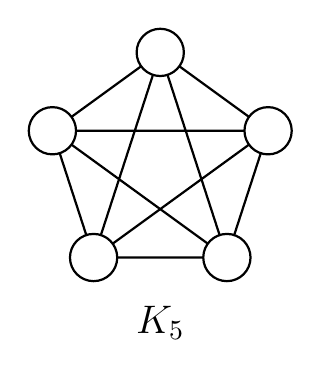
\begin{tikzpicture}[scale=0.8, baseline=(current bounding box.center)]
        % 定义样式:圆形节点,加粗黑边,白色填充
        \tikzstyle{vnode}=[circle, draw=black, thick, fill=white, minimum size=6mm, inner sep=0pt]
        
        % 定义 K5 的 5 个顶点坐标 (90度开始,每72度一个)
        \foreach \i in {1,...,5} {
            \coordinate (n\i) at (18+72*\i:1.8);
        }
        
        % 画边:两两相连
        % 技巧:先画五边形,再画内部五角星
        \draw[thick] (n1) -- (n2) -- (n3) -- (n4) -- (n5) -- cycle; % 五边形
        \draw[thick] (n1) -- (n3) -- (n5) -- (n2) -- (n4) -- cycle; % 五角星
        
        % 画节点 (覆盖在连线上方)
        \foreach \i in {1,...,5} {
            \node[vnode] at (n\i) {};
        }
        
        % 底部文字
        \node at (0, -2.5) {\Large $K_5$};
    \end{tikzpicture}
    \hspace{2cm} % 左右图之间的间距
    % === 右图 K3,3 ===
    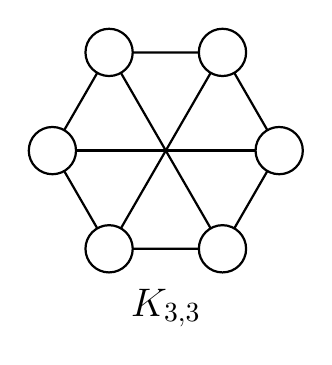
\begin{tikzpicture}[scale=0.8, baseline=(current bounding box.center)]
        \tikzstyle{vnode}=[circle, draw=black, thick, fill=white, minimum size=6mm, inner sep=0pt]
        
        % 定义 K3,3 的 6 个顶点坐标 (正六边形)
        \foreach \i in {1,...,6} {
            \coordinate (u\i) at (60*\i-60:1.8);
        }
        
        % 画边:
        % 1. 外部六边形 (连接相邻点)
        \draw[thick] (u1)--(u2)--(u3)--(u4)--(u5)--(u6)--cycle;
        
        % 2. 内部对角线 (连接对立点)
        \draw[thick] (u1)--(u4);
        \draw[thick] (u2)--(u5);
        \draw[thick] (u3)--(u6);
        
        % 画节点
        \foreach \i in {1,...,6} {
            \node[vnode] at (u\i) {};
        }
        
        % 底部文字
        \node at (0, -2.5) {\Large $K_{3,3}$};
    \end{tikzpicture}
    
    \caption{左图是 $K_5$,右图是 $K_{3,3}$,这是它们的一种比较有对称性的画法,而且最重要的是,我要突出它们都是哈密顿图,即存在一个经过所有点的回路}
\end{figure}

此外,本文的证明框架采用了 Carsten Thomassen 于 1980 年提出的经典技巧。请务必记住这个名字,因为正是得益于他的贡献,我们才避开了极其繁琐的拓扑讨论。

\section{必要性证明}

必要性的证明主要是证明 $K_5$ 和 $K_{3,3}$ 不是平面图。

\subsection{基于平面图的欧拉公式的证明}

如果我们引用欧拉公式,有一个十分简单的代数证明,由于欧拉公式指出,对于一个点数为 $n$ ,边数为 $e$ ,面数为 $f$ 的连通平面图,必有 $n-e+f=2$ ,而在平面简单图中,每个面至少需要三条边围成( $2f\le 3e$ ),也就有 $e\le 3n-6$ ;对于平面二分简单图,由于不存在奇环,每个面至少要四条边围成( $2f\le 4e$ ),也就有 $e\le 2n-4$ 。

然而,对于这两个简单图, $K_5$ 的边数为 10 ,点数为 5 ,刚好不满足 $e\le 3n-6$ ; $K_{3,3}$ 的边数为 9 ,点数为 6 ,刚好不满足 $e\le 2n-4$ ,因此,由欧拉公式,它们不可能是平面图。

当然,为了我们后续的完整证明,应当采用更加本质的证明方法,即基于圈弦的证明方法。

\subsection{基于圈弦的证明}

它的证明思路如下:对于任意一个存在哈密顿回路的图 $G$ ,实际上有一个简单的办法来判断这个图是不是平面图,那就是取出这个图的哈密顿回路 $P$ ,假设 $G$ 存在平面嵌入,它的哈密顿回路在平面上必然把平面分割成内部和外部,不妨设点的序列是 $v_1,v_2,\cdots,v_n$ ,那么其它不在哈密顿回路上的边(我们称为弦)要么完全在内部、要么完全在外部。

\begin{figure}[H]
    \centering
    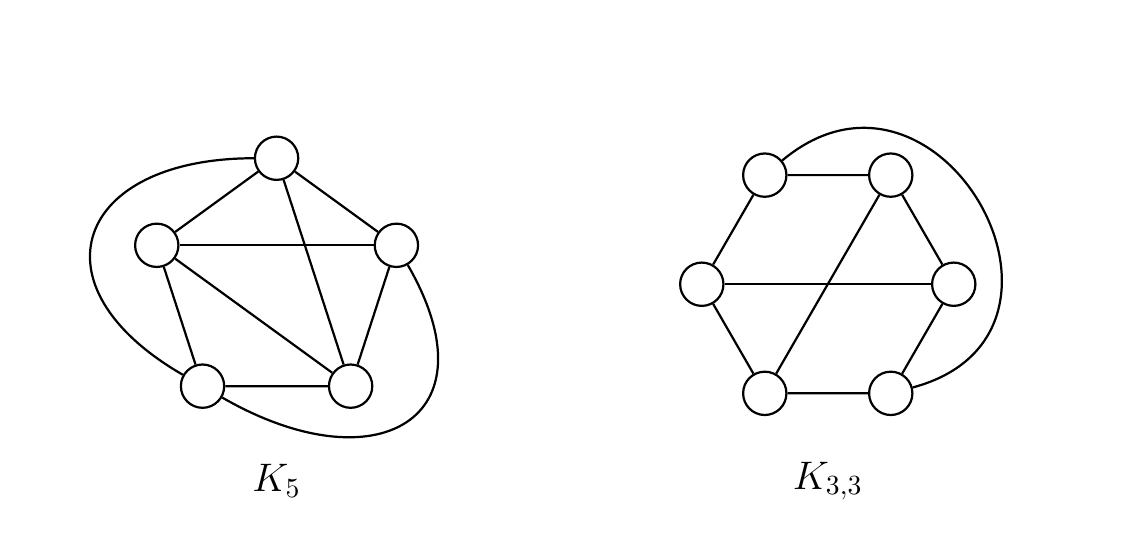
\begin{tikzpicture}[scale=1, auto, swap]
        % ================= 样式定义 =================
        \tikzset{
            vnode/.style={circle, draw=black, thick, fill=white, minimum size=5.5mm, inner sep=0pt},
            edge/.style={thick, black}
        }

        % ================= 左图:K5 =================
        \begin{scope}[shift={(-3.5,0)}]
            % 顶点:正五边形,顶角朝上
            \node[vnode] (n1) at (90:1.6) {};   % 顶
            \node[vnode] (n2) at (162:1.6) {};  % 左上
            \node[vnode] (n3) at (234:1.6) {};  % 左下
            \node[vnode] (n4) at (306:1.6) {};  % 右下
            \node[vnode] (n5) at (18:1.6) {};   % 右上

            % 边
            \draw[edge] (n1)--(n2)--(n3)--(n4)--(n5)--(n1);
            \draw[edge] (n1)--(n4);
            \draw[edge] (n2)--(n4);
            \draw[edge] (n2)--(n5);
            %\draw[edge] (n3)--(n5);

            % 【修正】外部曲线
            % out=130: 往左上方大角度出去
            % in=150:  从左上方大角度进来
            % 这样保证弧线完全在左侧外部,是一个饱满的“C”形
            \draw[edge] (n1) to[out=180, in=150, looseness=2] (n3);
            \draw[edge] (n3) to[out=330, in=300, looseness=2] (n5);

            \node at (0, -2.5) {\Large $K_5$};
        \end{scope}

        % ================= 右图:K3,3 =================
        \begin{scope}[shift={(3.5,0)}]
            % 顶点:正六边形,平顶
            \node[vnode] (u1) at (120:1.6) {}; % 左上
            \node[vnode] (u2) at (60:1.6) {};  % 右上
            \node[vnode] (u3) at (0:1.6) {};   % 右
            \node[vnode] (u4) at (300:1.6) {}; % 右下
            \node[vnode] (u5) at (240:1.6) {}; % 左下
            \node[vnode] (u6) at (180:1.6) {}; % 左

            % 边
            \draw[edge] (u1)--(u2)--(u3)--(u4)--(u5)--(u6)--(u1);
            \draw[edge] (u6)--(u3);
            \draw[edge] (u5)--(u2);

            % 【修正】外部曲线
            % out=75:  向右上方飞出,避开顶部
            % in=110:  【重点】改为斜向切入,绝对不是垂直向下(90)
            % 这样线条会以自然的斜率穿过中间区域,视觉上不会造成歧义
            \draw[edge] (u1) to[out=40, in=15, looseness=2] (u4);

            \node at (0, -2.5) {\Large $K_{3,3}$};
        \end{scope}

    \end{tikzpicture}
    \caption{如图所示,下面是 $K_5$ 和 $K_{3,3}$ 的演示,弦可以画在圈的外部或者内部}
\end{figure}

那么,不妨设两条弦 $(x_i,x_j),(x_k,x_l)$ ,那么我们声明如果 $i < k < j < l$ ,那么如果这两条弦被同时画在内部或外部,它们必然会相交;这里不给出涉及拓扑的严格证明,但从直观理解仍然显然,你可以用圆中弦和弧的对应来直观理解这个命题的正确性,即对于空间(也许是圈的内部或外部) $v_i$ 到 $v_j$ 在圈上的路径和它们的连边又把这个空间分成了两个区域,其中 $v_k,v_l$ 正是分别处于这两个区域,因此它们的连边必然与某条边交叉。

\begin{figure}[H]
    \centering
    \begin{tikzpicture}[scale=1, auto, swap]
        % ================= 样式定义 =================
        \tikzset{
            % 节点:增加 font 设置以便显示 v1, v2...
            vnode/.style={circle, draw=black, thick, fill=white, minimum size=6mm, inner sep=0pt, font=\small},
            edge/.style={thick, black}
        }

        % ================= 左图:外部弦不相交演示 =================
        \begin{scope}[shift={(-3.5,0)}]
            % 1. 定义顶点 (正五边形, 顺时针编号)
            % v1(顶), v2(右), v3(右下), v4(左下), v5(左)
            \node[vnode] (v1) at (90:1.6) {$v_1$};
            \node[vnode] (v2) at (18:1.6) {$v_2$};
            \node[vnode] (v3) at (306:1.6) {$v_3$};
            \node[vnode] (v4) at (234:1.6) {$v_4$};
            \node[vnode] (v5) at (162:1.6) {$v_5$};

            % 2. 绘制基础圈 (Cycle)
            \draw[edge] (v1)--(v2)--(v3)--(v4)--(v5)--(v1);
            \draw[edge] (n1)--(n4);
            \draw[edge] (n2)--(n4);
            \draw[edge] (n2)--(n5);
            % 3. 绘制外部弦 (演示不相交)
            % 弦 1: (v1, v4) -> 从左侧绕行 (out=180, in=150)
            \draw[edge] (v1) to[out=180, in=150, looseness=1.8] (v4);
            
            % 弦 2: (v2, v4) -> 从下方绕行 (out=-60, in=-30)
            % 这样两条线虽然终点相同,但在路径上没有“交叉”
            \draw[edge] (v2) to[out=-60, in=-30, looseness=1.8] (v4);
            
            \node at (0, -2.5) {\Large $K_5$};

        \end{scope}

        % ================= 右图:内部弦相交演示 =================
        \begin{scope}[shift={(3.5,0)}]
            % 1. 定义顶点 (正六边形, 顺时针编号, 平顶布局匹配 K3,3)
            % v1(左上), v2(右上), v3(右), v4(右下), v5(左下), v6(左)
            \node[vnode] (u1) at (120:1.6) {$v_1$};
            \node[vnode] (u2) at (60:1.6) {$v_2$};
            \node[vnode] (u3) at (0:1.6) {$v_3$};
            \node[vnode] (u4) at (300:1.6) {$v_4$};
            \node[vnode] (u5) at (240:1.6) {$v_5$};
            \node[vnode] (u6) at (180:1.6) {$v_6$};

            % 2. 绘制基础圈 (Cycle)
            \draw[edge] (u1)--(u2)--(u3)--(u4)--(u5)--(u6)--(u1);

            % 3. 绘制内部弦 (演示相交)
            % (v2, v5) 连接右上和左下
            \draw[edge] (u2) -- (u5);
            
            % (v3, v6) 连接右和左
            \draw[edge] (u3) -- (u6);
            
            % 显而易见,这两条线在中心相交
            \draw[edge] (u1) to[out=40, in=15, looseness=2] (u4);
            
            \node at (0, -2.5) {\Large $K_{3,3}$};
        \end{scope}

    \end{tikzpicture}
    \caption{如图所示,对点进行了标号,方便检验与直观理解,比如右图 $(v_2,v_5)$ $(v_3,v_6)$ 都被画在内部,而且相交;而左图 $(v_2,v_4)$ $(v_1,v_4)$ 都被画在外部,且不相交}
\end{figure}

那么,显然,将弦看作点,得到一个新图;原图对应弦如果“必然会相交”,那就在新图对应的顶点连边。

现在问题就转换成,能否把新图的所有顶点进行黑白染色,使得一条边不会连接两个同色点,那么这是经典的二分图判定问题,我们可以容易地得到,对于 $K_5$ 和 $K_{3,3}$ ,它们基于弦构建的新图并不是二分图(包含一个长度为 5 的环和一个长度为 3 的环),也就证明了它们不是平面图。

然后接下来我们定义一个图的细分为在图的边上加入若干顶点形成的图。那么,图的细分并不会改变图是不是一个平面图,如果你画出了一个平面图,你把其中一条边变为长长的路径会改变它能否画在一个平面上嘛?当然不会!

所以,图 $G$ 是平面图当且仅当它的细分是平面图。

好那么,如果一个图 $G$ 可以被画在平面上,而且包含一个 $K_5$ 或 $K_{3,3}$ 的细分作为子图。

反证法:那么假设这个图 $G$ 可以画在平面上,它的任意子图,显然也是可以画在平面上的,因为直观来看,你只需要去掉一些顶点和边就可以得到它的任意子图了,你不需要改变画法也不会引入相交。

因此 $K_5$ 或 $K_{3,3}$ 的细分是平面图,也就是说 $K_5$ 或 $K_{3,3}$ 是平面图,但是我们已经证明了,它们不是平面图。

好的那么 $G$ 不是平面图,也就证明了 Kuratowski 定理的必要性。接下来我们证明充分性。

\section{连通性归约}

数学家们证明反例不存在的时候,有时候会用一种类似耍流氓的做法:你配做我的反例嘛!

简单来说,如果一个反例能够归约为一个更小的反例,数学家们就声称可以被归约到更小的反例是“不配做反例的”;然后嘛……数学家们归约一下发现,没办法找到配做反例的了,然后就证明没有反例。

这一般是很有效的,因为可能的图太多了,数学家们需要集中精力针对一小撮。

那么 Kuratowski 定理的充分性整体上就是这样,我们假设存在这样一个反例 $G$ (不包含 $K_5$ 或 $K_{3,3}$ 的细分,且不是平面图),我们声称,只有边数最少(在此基础上点数要最少)的 $G$ 才配做反例!边数更多的不配!

我们最终当然是希望证明 $G$ 不存在,但这一节要证明这样的 $G$ 一定是 3-连通的,即强行删掉两个点 $G$ 仍然连通。

\subsection{不连通的情况}
首先排除 $G$ 不连通的情况,因为如果是这样,由于 $G$ 是最小的反例,它的每个连通分量都是平面图,那么把每个连通分量分开画出来不就相当于把 $G$ 画在平面上了?所以 $G$ 如果存在必然连通。

\begin{figure}[H]
    \centering
    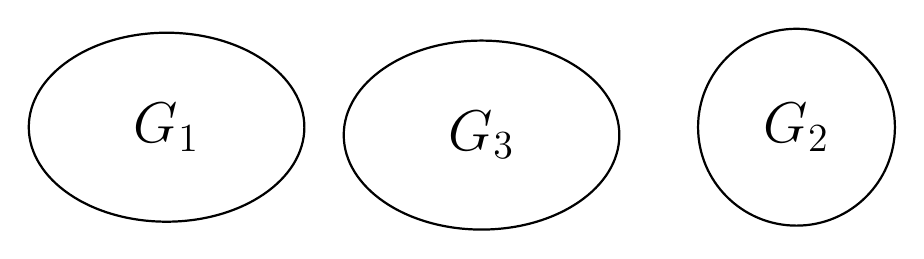
\begin{tikzpicture}[scale=1]
        % ================= 样式定义 =================
        % 连通分量样式:黑边,加粗,白色填充,大字体
        \tikzset{
            blob/.style={draw=black, thick, fill=white, align=center, font=\huge}
        }

        % ================= 绘图部分 =================
        
        % G1: 左上,椭圆 (ellipse)
        % minimum width/height 控制椭圆的长宽
        \node[blob, ellipse, minimum width=3.5cm, minimum height=2.4cm] at (-4, 0) {$G_1$};

        % G2: 右上,圆形 (circle)
        % minimum size 控制直径
        \node[blob, circle, minimum size=2.5cm] at (4, 0) {$G_2$};

        % G3: 下方居中,椭圆
        \node[blob, ellipse, minimum width=3.5cm, minimum height=2.4cm] at (0, -0.1) {$G_3$};

    \end{tikzpicture}
    \caption{如图,把 $G_1, G_2, G_3$ 等连通分量分开画即可}
\end{figure}

\subsection{1-连通的情况}
接着排除 $G$ 的点连通度为 1 的情况,因为 $G$ 是 1 连通意味着有割点,任取一个割点 $v$ ,然后去掉这个割点,得到若干连通分量,再按原来的连边方式在每个连通分量加上这个割点,得到 $G_1,G_2,\cdots,G_c$ ,由于 $G$ 是最小反例,且每个连通分量至少比原来少一条边,所以每个连通分量都是平面图。

这里需要一个引理,我们可以证明,对于任意平面图的一种画法,对于原画法中的任何一个有界面,存在另一种画法,使得该有界面在新画法中对应着无界面。

\begin{figure}[H]
    \centering
    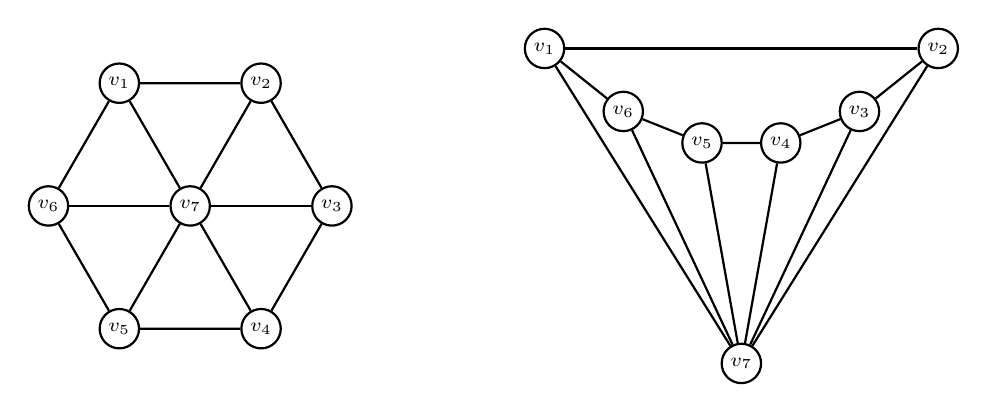
\begin{tikzpicture}[scale=1, auto, swap]
        % ================= 样式定义 =================
        \tikzset{
            % 节点:稍微小一点,以容纳文字,字体设为 \scriptsize
            vnode/.style={circle, draw=black, thick, fill=white, minimum size=5mm, inner sep=0pt, font=\scriptsize},
            edge/.style={thick, black}
        }

        % ================= 左图:轮图 (Hexagon Wheel) =================
        \begin{scope}[shift={(-3.5,0)}]
            % 1. 中心点 v7
            \node[vnode] (v7) at (0,0) {$v_7$};

            % 2. 外圈顶点 (逆时针或顺时针布局)
            % 根据原图视觉:v1在左上,v2在右上 -> 对应角度约为 120度和 60度
            % 顺序:v1(120), v2(60), v3(0), v4(300), v5(240), v6(180)
            \node[vnode] (v1) at (120:1.8) {$v_1$};
            \node[vnode] (v2) at (60:1.8)  {$v_2$};
            \node[vnode] (v3) at (0:1.8)   {$v_3$};
            \node[vnode] (v4) at (300:1.8) {$v_4$};
            \node[vnode] (v5) at (240:1.8) {$v_5$};
            \node[vnode] (v6) at (180:1.8) {$v_6$};

            % 3. 绘制外圈连边
            \draw[edge] (v1)--(v2)--(v3)--(v4)--(v5)--(v6)--(v1);

            % 4. 绘制辐条 (中心向外)
            \foreach \x in {v1,v2,v3,v4,v5,v6} {
                \draw[edge] (v7) -- (\x);
            }
        \end{scope}

        % ================= 右图:投影变换 (Projection) =================
        \begin{scope}[shift={(3.5,0)}]
            % 布局逻辑:
            % v1, v2 拉宽放在顶部
            % v7 放在最底部
            % v6-v5-v4-v3 形成一个悬垂的微笑曲线

            % 1. 关键锚点
            \node[vnode] (u1) at (-2.5, 2)  {$v_1$}; % 左上
            \node[vnode] (u2) at (2.5, 2)   {$v_2$}; % 右上
            \node[vnode] (u7) at (0, -2)    {$v_7$}; % 底部

            % 2. 中间链条点 (手动设定坐标以形成弧度)
            \node[vnode] (u6) at (-1.5, 1.2) {$v_6$};
            \node[vnode] (u5) at (-0.5, 0.8) {$v_5$};
            \node[vnode] (u4) at (0.5, 0.8)  {$v_4$};
            \node[vnode] (u3) at (1.5, 1.2)  {$v_3$};

            % 3. 绘制顶部边 (原图中的 v1-v2)
            \draw[edge] (u1) -- (u2);

            % 4. 绘制悬垂链条 v1-v6-v5-v4-v3-v2
            \draw[edge] (u1) -- (u6) -- (u5) -- (u4) -- (u3) -- (u2);

            % 5. 绘制辐条 (所有点都连向 v7)
            \foreach \x in {u1,u2,u3,u4,u5,u6} {
                \draw[edge] (u7) -- (\x);
            }
        \end{scope}

    \end{tikzpicture}
    \caption{如图所示,$v_1-v_2-v_7$ 在左图是有界面,在右图是无界面}
\end{figure}

这是一个有关于球极投影的定理,我这里给出它的直观理解,简单来说,对于任意一个平面图 $G$ ,它既然可以画在平面上,那么它就可以画在球面上,而球面上没有内部面和外部面之分。

然后如果我们想要一个有界面成为新图的无界面,我们就把它画在球面上的那个空白位置戳一个洞,然后扯开铺平即可。

好那么对于我们的 $G_1,G_2,\cdots,G_c$ ,这意味着总是存在一种画法让 $v$ 出现在外部面,那么我们直接把它们的 $v$ 像花瓣一样合在一起即可给出 $G$ 的平面嵌入:

\begin{figure}[H]
    \centering
    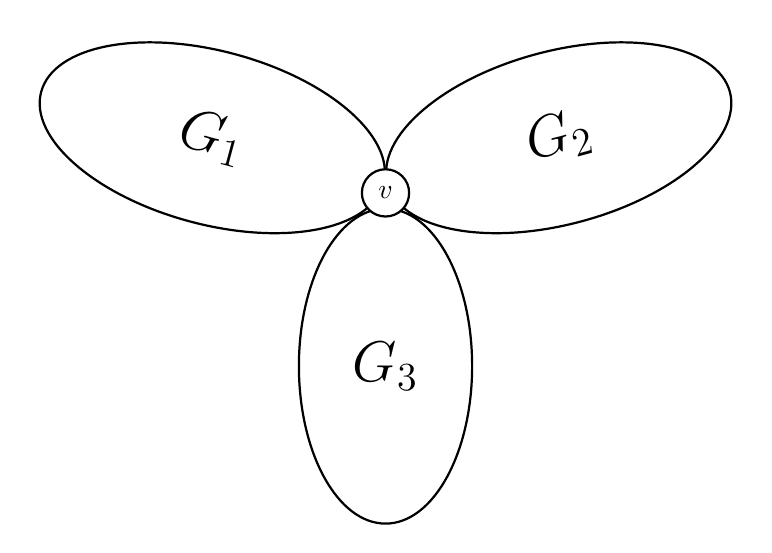
\begin{tikzpicture}[scale=1]
        % ================= 样式定义 =================
        \tikzset{
            % 椭圆区域样式:白底黑边,文字大
            blob/.style={draw=black, thick, fill=white, align=center, font=\huge},
            % 割点 v 的样式
            vnode/.style={circle, draw=black, thick, fill=white, minimum size=6mm, inner sep=0pt, font=\normalsize}
        }

        % ================= 绘图部分 =================
        
        % 技巧:先画椭圆,最后画中间的 v 点,这样 v 会覆盖掉椭圆交叉的线条
        
        % G1: 左上花瓣 (旋转椭圆)
        % rotate=15 让它稍微翘起来一点
        \node[blob, ellipse, minimum width=4.5cm, minimum height=2.2cm, rotate=-15] 
            at (-2.2, 0.7) {$G_1$};

        % G2: 右上花瓣
        % rotate=-15 让它往另一边翘
        \node[blob, ellipse, minimum width=4.5cm, minimum height=2.2cm, rotate=15] 
            at (2.2, 0.7) {$G_2$};

        % G3: 下方花瓣
        % 垂直椭圆
        \node[blob, ellipse, minimum width=2.2cm, minimum height=4cm] 
            at (0, -2.2) {$G_3$};

        % v: 中心割点 (画在最上层)
        \node[vnode] (v) at (0,0) {$v$};

    \end{tikzpicture}
    \caption{如图,确实很像花瓣} 
\end{figure}

那么 $G$ 如果存在则的点连通度至少为 2。

\subsection{2-连通的情况}
接着我们考虑点连通度为 2 的情况,这意味着 $G$ 存在两个顶点的割集 $\{x,y\}$ ,好的接下来我们将 $G$ 去掉这两个顶点 $x,y$ 得到若干连通分支,然后再将这两个顶点粘合回去(继承原本 $x,y$ 的连边方式),得到连通分支 $G_1,G_2,\cdots,G_c$ 。

首先这每个连通分支单独来看,都是与原来的 $x,y$ 都分别相连的,不然单独去掉 $x,y$ 中的一个它们就会分离出来,图就不是 2-连通的了,这意味着,我们得到的每个连通分支,边数都至少比原来的 $G$ 要少两条。

接下来我们执行粘合操作,先考虑 $G_1,G_2$ ,如果 $x,y$ 原本在 $G$ 中没有连边,让它们在 $G_1,G_2$ 中先临时连边,否则不动,令这样操作后得到的连通图为 $G_1^+,G_2^+$ ,由于它们只是多了一条边,还是比 $G$ 边数少,由于 $G$ 是最小反例,所以 $G_1^+,G_2^+$ 仍然都是平面图。

这里有一个极其容易忽略的细节(包括我一开始的写作都忽略了)我们之前论证的完整逻辑是:
\begin{enumerate}
    \item 因为 $G$ 不包含 $K_5$ 或 $K_{3,3}$ 的细分作为子图,所以 $G_1$ 也不包含 $K_5$ 或 $K_{3,3}$ 的细分作为子图。
    \item 如果 $G_1$ 不是平面图,那么由于 $G_1$ 不包含 $K_5$ 或 $K_{3,3}$ 的细分作为子图,它的边数小于 $G$ ,它会是一个更小的反例。
\end{enumerate}

但在这里 $G_1^+$ 确实更小,但有没有可能(当 $x,y$ 原本没有连边时,因为加入了边)包含 $K_5$ 或 $K_{3,3}$ 的细分作为子图呢?不可能,证明考虑反证法,如果出现这种情况,那么这个细分子图一定包含加入的这条边,那么由于 $G_2$ 是连通的,我们可以用 $G_2$ 上的 $x,y$ 路径替换这个强行加入的边,那么就可以证明 $G$ 包含 $K_5$ 或 $K_{3,3}$ 的细分作为子图,矛盾。

因此 $G_1^+$ 不包含 $K_5$ 或 $K_{3,3}$ 的细分作为子图,同理 $G_2^+$ 也是,这样才能继续证明它们是平面图。

那么由于之前的球面投影论证,它们都存在一个平面嵌入,可以把 $x,y$ 连边放到外部面的边缘,将其沿着 $x,y$ 连边粘合,得到一个新图的平面嵌入。

\begin{figure}[H]
    \centering
    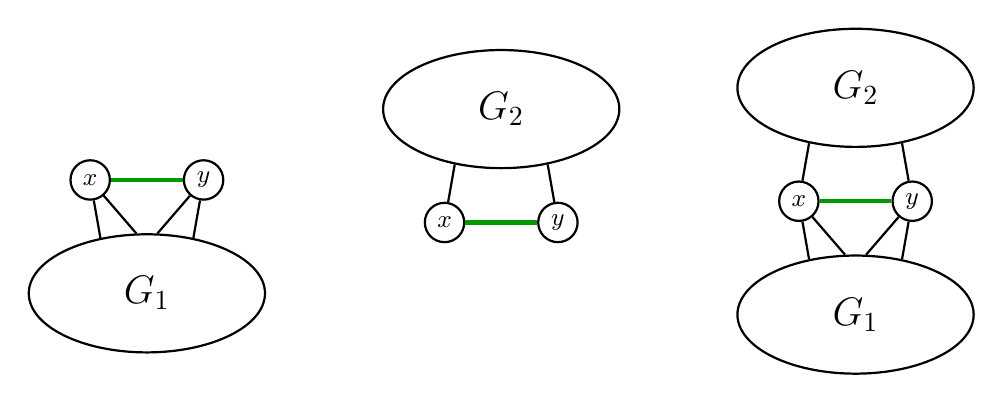
\begin{tikzpicture}[scale=0.9, auto, swap]
        % ================= 样式定义 =================
        \tikzset{
            % 连通块样式:椭圆
            blob/.style={draw=black, thick, fill=white, align=center, font=\Large},
            % 节点样式:小圆圈
            vnode/.style={circle, draw=black, thick, fill=white, minimum size=5mm, inner sep=0pt, font=\small},
            % 普通边
            edge/.style={thick, black},
            % 强调边 (绿色)
            newedge/.style={ultra thick, green!60!black}
        }

        % ================= 第一部分:G1 (左) =================
        \begin{scope}[shift={(-5, -0.5)}]
            % G1 椭圆主体
            \node[blob, ellipse, minimum width=3cm, minimum height=1.5cm] (g1) at (0, -0.8) {$G_1$};
            
            % 节点 x, y (悬浮在上方)
            \node[vnode] (x1) at (-0.8, 0.8) {$x$};
            \node[vnode] (y1) at (0.8, 0.8) {$y$};
            
            % 连接腿 (Legs)
            % 从 x 连向 G1 的左上侧
            \draw[edge] (x1) -- (g1.130);
            \draw[edge] (x1) -- (g1.100);
            % 从 y 连向 G1 的右上侧
            \draw[edge] (y1) -- (g1.50);
            \draw[edge] (y1) -- (g1.80);
            
            % 绿边
            \draw[newedge] (x1) -- (y1);
        \end{scope}

        % ================= 第二部分:G2 (中) =================
        \begin{scope}[shift={(0, 0.5)}]
            % G2 椭圆主体 (悬浮在上方)
            \node[blob, ellipse, minimum width=3cm, minimum height=1.5cm] (g2) at (0, 0.8) {$G_2$};
            
            % 节点 x, y (悬浮在下方)
            \node[vnode] (x2) at (-0.8, -0.8) {$x$};
            \node[vnode] (y2) at (0.8, -0.8) {$y$};
            
            % 连接腿
            % 从 x 连向 G2 的左下侧
            \draw[edge] (x2) -- (g2.230);
            % 从 y 连向 G2 的右下侧
            \draw[edge] (y2) -- (g2.310);
            
            % 绿边
            \draw[newedge] (x2) -- (y2);
        \end{scope}

        % ================= 第三部分:粘合结果 (右) =================
        \begin{scope}[shift={(5, 0)}]
            % 节点 x, y (位于中心)
            \node[vnode] (x3) at (-0.8, 0) {$x$};
            \node[vnode] (y3) at (0.8, 0) {$y$};
            
            % --- 上方 G2 ---
            \node[blob, ellipse, minimum width=3cm, minimum height=1.5cm] (g2_final) at (0, 1.6) {$G_2$};
            \draw[edge] (x3) -- (g2_final.230);
            \draw[edge] (y3) -- (g2_final.310);
            
            % --- 下方 G1 ---
            \node[blob, ellipse, minimum width=3cm, minimum height=1.5cm] (g1_final) at (0, -1.6) {$G_1$};
            \draw[edge] (x3) -- (g1_final.130);
            \draw[edge] (x3) -- (g1_final.100);
            \draw[edge] (y3) -- (g1_final.50);
            \draw[edge] (y3) -- (g1_final.80);
            
            % 绿边 (作为接口)
            \draw[newedge] (x3) -- (y3);
        \end{scope}

    \end{tikzpicture}
    \caption{如图所示,上面显示了一个典型的 $G_1$ $G_2$ 粘合的场景,绿边是强行加入的边,由于 $G_1^+$ 和 $G_2^+$ 都是平面图,粘合是可行的}
\end{figure}

那么这个粘合后的结果由于是平面图,仍然可以把 $x,y$ 的一条连边放到其外部面的边缘,如此,便可以把所有连通块都粘合在一起,得到一个平面图。

\begin{figure}[H]
    \centering
    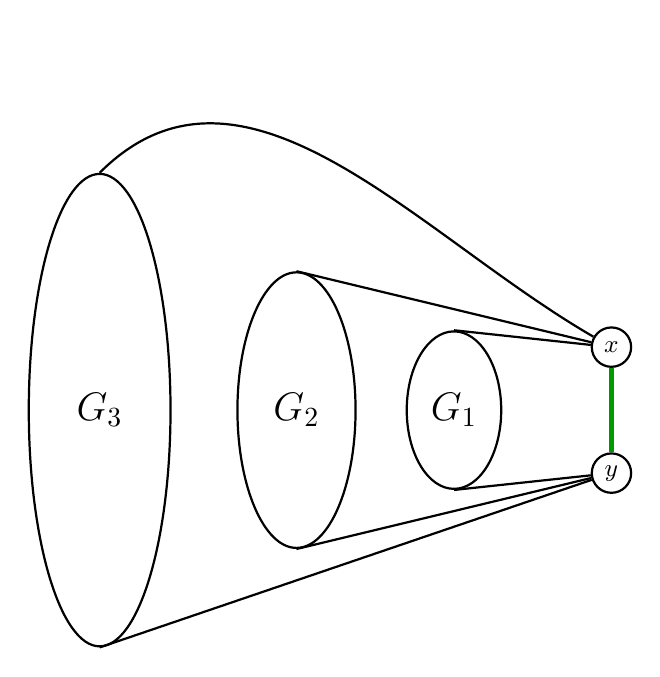
\begin{tikzpicture}[scale=1, auto, swap]
        % ================= 样式定义 =================
        \tikzset{
            % 椭圆样式:白底黑边
            blob/.style={draw=black, thick, fill=white, align=center, font=\Large},
            % 节点样式
            vnode/.style={circle, draw=black, thick, fill=white, minimum size=5mm, inner sep=0pt, font=\small},
            % 边样式
            edge/.style={thick, black},
            % 绿色强调边
            newedge/.style={ultra thick, green!60!black}
        }

        % ================= 1. 绘制椭圆节点 =================
        
        % G3: 最左边,最高最瘦
        \node[blob, ellipse, minimum width=1.8cm, minimum height=6cm] (g3) at (0, 0) {$G_3$};

        % G2: 中间,中等高度
        \node[blob, ellipse, minimum width=1.5cm, minimum height=3.5cm] (g2) at (2.5, 0) {$G_2$};

        % G1: 右边,最矮
        \node[blob, ellipse, minimum width=1.2cm, minimum height=2cm] (g1) at (4.5, 0) {$G_1$};

        % x, y: 最右侧的端点
        \node[vnode] (x) at (6.5, 0.8) {$x$};
        \node[vnode] (y) at (6.5, -0.8) {$y$};

        % ================= 2. 绘制连线 =================

        % --- G1 的连线 (最内层) ---
        \draw[edge] (g1.north) -- (x);
        \draw[edge] (g1.south) -- (y);

        % --- G2 的连线 (中间层) ---
        % 稍微弯曲一点,体现层次感
        \draw[edge] (g2.north) -- (x);
        \draw[edge] (g2.south) -- (y);

        % --- G3 的连线 (最外层) ---
        % 关键:顶部的线要画出“包覆”的大弧度
        % out=45, in=135 让线条向上拱起
        \draw[edge] (g3.north) to[out=45, in=150] (x);
        % 底部的线相对平直
        \draw[edge] (g3.south) -- (y);

        % ================= 3. 绘制绿边 =================
        \draw[newedge] (x) -- (y);

    \end{tikzpicture}
    \caption{如图显示了粘合之后仍然可以把 $x-y$ 连边放到外部面的状态}
\end{figure}

此时,如果 $G$ 中 $x,y$ 本没有连边,去掉新图的 $x,y$ 连边,否则不变。

由此可以得到 $G$ 的一个平面嵌入,也就证明了 $G$ 是平面图。

因此 $G$ 的点连通度至少为 3。

好么,那么你可不可以说明 $G$ 的点连通度不能是 3 呢?实际上是不行的,因为 $K_{3,3}$ 的点连通度恰好就是 3,我们的目标其实是归约来证明 $G$ 在收缩到极小(不能通过一些显然的变换变得更小)时,要么是 $K_5$ ,要么是 $K_{3,3}$ ,所以,基于连通性的归约到此结束了。

当然,我们费劲归约到 3-连通图实际上并不是毫无作用的,我们很快就可以看到这点。

\section{2-连通平面图的性质}

我们要证明 2-连通平面图的任意一个面的边界一定是一个圈(也就是,它可以由一个不经过重复的顶点和边回路遍历),为什么呢?因为对于非连通平面图和 1-连通图,这个性质不一定成立。

\begin{figure}[H]
    \centering
    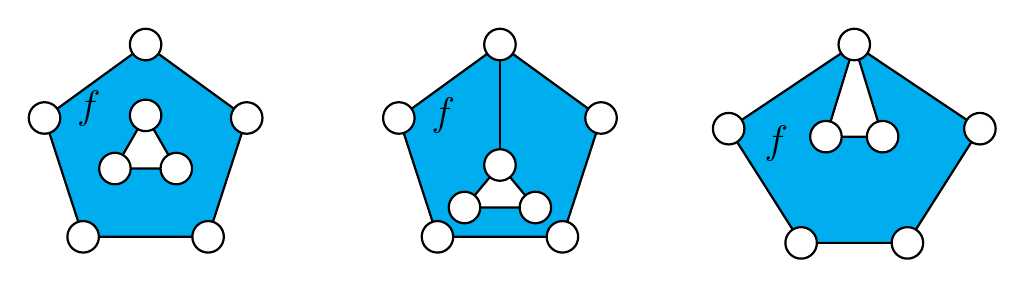
\begin{tikzpicture}[scale=0.9, auto, swap]
        % ================= 样式定义 =================
        \tikzset{
            % 节点样式
            vnode/.style={circle, draw=black, thick, fill=white, minimum size=4mm, inner sep=0pt},
            % 边样式
            edge/.style={thick, black},
            % 面 f 的填充样式 (关键:even odd rule 用于挖洞)
            facefill/.style={fill=cyan, even odd rule}
        }

        % ================= 1. 左上:不连通 (Disconnected) =================
        \begin{scope}[shift={(-5, 0)}]
            % 定义外圈坐标 (五边形)
            \coordinate (o1) at (90:1.5);
            \coordinate (o2) at (162:1.5);
            \coordinate (o3) at (234:1.5);
            \coordinate (o4) at (306:1.5);
            \coordinate (o5) at (18:1.5);

            % 定义内圈坐标 (倒三角形)
            \coordinate (i1) at (90:0.5); % 稍微下移一点不重合
            \coordinate (i2) at (210:0.5);
            \coordinate (i3) at (330:0.5);

            % 步骤 A: 填充蓝色区域 (挖洞)
            % 语法:(外圈路径) (内圈路径)
            \fill[facefill] (o1)--(o2)--(o3)--(o4)--(o5)--cycle 
                            (i1)--(i2)--(i3)--cycle;

            % 步骤 B: 绘制边
            \draw[edge] (o1)--(o2)--(o3)--(o4)--(o5)--cycle;
            \draw[edge] (i1)--(i2)--(i3)--cycle;

            % 步骤 C: 绘制节点 (必须最后画,盖住线头)
            \foreach \p in {o1,o2,o3,o4,o5,i1,i2,i3} \node[vnode] at (\p) {};

            % 标签 f
            \node[font=\Large] at (-0.8, 0.6) {$f$};
        \end{scope}

        % ================= 2. 左下:有割边 (Cut Edge / Bridge) =================
        \begin{scope}[shift={(0, 0)}]
            % 外圈 (五边形)
            \coordinate (o1) at (90:1.5);
            \coordinate (o2) at (162:1.5);
            \coordinate (o3) at (234:1.5);
            \coordinate (o4) at (306:1.5);
            \coordinate (o5) at (18:1.5);

            % 内圈 (三角形)
            \coordinate (i1) at (0, -0.2); 
            \coordinate (i2) at (-0.5, -0.8);
            \coordinate (i3) at (0.5, -0.8);

            % A. 填充
            \fill[facefill] (o1)--(o2)--(o3)--(o4)--(o5)--cycle 
                            (i1)--(i2)--(i3)--cycle;

            % B. 绘制边
            \draw[edge] (o1)--(o2)--(o3)--(o4)--(o5)--cycle;
            \draw[edge] (i1)--(i2)--(i3)--cycle;
            % 【关键】割边:连接外圈 o1 和内圈 i1
            \draw[edge] (o1) -- (i1);

            % C. 绘制节点
            \foreach \p in {o1,o2,o3,o4,o5,i1,i2,i3} \node[vnode] at (\p) {};
            
            % 标签 f
            \node[font=\Large] at (-0.8, 0.5) {$f$};
        \end{scope}

        % ================= 3. 右侧:有割点 (Cut Vertex) =================
        \begin{scope}[shift={(5, 0)}]
            % 共享顶点 top
            \coordinate (top) at (90:1.5);

            % 外圈其余点 (扁五边形)
            \coordinate (o2) at (170:1.8);
            \coordinate (o3) at (240:1.5);
            \coordinate (o4) at (300:1.5);
            \coordinate (o5) at (10:1.8);

            % 内圈其余点 (悬挂在 top 下方的三角形)
            \coordinate (i2) at (-0.4, 0.2);
            \coordinate (i3) at (0.4, 0.2);

            % A. 填充
            % 注意:内圈路径必须包含 shared vertex (top)
            \fill[facefill] (top)--(o2)--(o3)--(o4)--(o5)--cycle 
                            (top)--(i2)--(i3)--cycle;

            % B. 绘制边
            \draw[edge] (top)--(o2)--(o3)--(o4)--(o5)--cycle;
            \draw[edge] (top)--(i2)--(i3)--cycle;

            % C. 绘制节点
            \foreach \p in {top,o2,o3,o4,o5,i2,i3} \node[vnode] at (\p) {};

            % 标签 f
            \node[font=\Large] at (-1.1, 0.1) {$f$};
        \end{scope}

    \end{tikzpicture}
    \caption{如图分别展示了图不连通,有割边和割点的特例,满足此时面 $f$ 的边界显然都不是圈}
\end{figure}

那么怎么证明呢?非常幸运的是,前人给了我们一个非常好用的工具,耳分解,它能够辅助我们用组合结构直观理解拓扑细节。

\subsection{耳分解引理必要性证明}

实际上,我们有图 $G$ 是 2-连通图当且仅当 $G$ 有耳分解。

$G$ 有耳分解的意思是, $G$ 可以由一个圈开始,逐步添加耳(即两端是原有的图中不同的两个端点,中间新增点和边的简单路径)得到。

\begin{figure}[H]
    \centering
    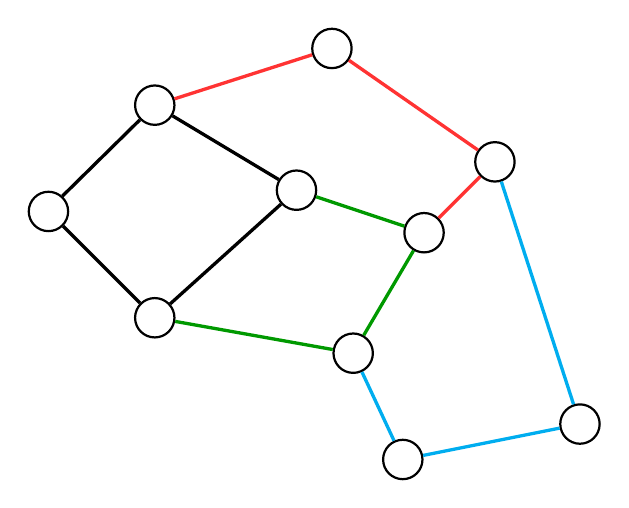
\begin{tikzpicture}[scale=0.9, auto, swap]
        % ================= 样式定义 =================
        \tikzset{
            % 节点:白底黑圈
            vnode/.style={circle, draw=black, thick, fill=white, minimum size=5mm, inner sep=0pt},
            % 边:统一加粗
            edge/.style={very thick}
        }

        % ================= 1. 黑色初始圈 (Initial Cycle) =================
        % 布局:类似菱形,稍微旋转
        \coordinate (n1) at (-1, 3);      % 顶
        \coordinate (n2) at (-2.5, 1.5);  % 左
        \coordinate (n3) at (-1, 0);      % 底
        \coordinate (n4) at (1, 1.8);     % 右(内)

        % 绘制黑色节点
        \node[vnode] (b1) at (n1) {};
        \node[vnode] (b2) at (n2) {};
        \node[vnode] (b3) at (n3) {};
        \node[vnode] (b4) at (n4) {};

        % 绘制黑色边
        \draw[edge, black] (b1) -- (b2) -- (b3) -- (b4) -- (b1);

        % ================= 2. 绿色耳 (Green Ear) =================
        % 连接黑色圈的底部(b3)和右侧(b4)
        \coordinate (cg1) at (1.8, -0.5); % 绿耳节点1
        \coordinate (cg2) at (2.8, 1.2);  % 绿耳节点2 (也是红耳的终点)

        \node[vnode] (g1) at (cg1) {};
        \node[vnode] (g2) at (cg2) {};

        \draw[edge, green!60!black] (b3) -- (g1) -- (g2) -- (b4);

        % ================= 3. 红色耳 (Red Ear) =================
        % 连接黑色圈的顶部(b1)和绿色耳的节点(g2)
        \coordinate (cr1) at (1.5, 3.8);  % 红耳节点1
        \coordinate (cr2) at (3.8, 2.2);  % 红耳节点2 (也是蓝耳的终点)

        \node[vnode] (r1) at (cr1) {};
        \node[vnode] (r2) at (cr2) {};

        \draw[edge, red!80] (b1) -- (r1) -- (r2) -- (g2);

        % ================= 4. 蓝色耳 (Blue Ear) =================
        % 连接绿色耳的节点(g1)和红色耳的节点(r2)
        \coordinate (cbl1) at (2.5, -2.0); % 蓝耳节点1
        \coordinate (cbl2) at (5.0, -1.5); % 蓝耳节点2

        \node[vnode] (bl1) at (cbl1) {};
        \node[vnode] (bl2) at (cbl2) {};

        \draw[edge, cyan] (g1) -- (bl1) -- (bl2) -- (r2);

    \end{tikzpicture}
    \caption{图示是一个图的耳分解,黑色边是初始的圈,红绿蓝色的边分别代表耳}
\end{figure}

这里出于需要我们只证明它的必要性,即 $G$ 是 2-连通图,则必有耳分解。

这是因为,既然 $G$ 是 2-连通的,它必然有一个简单回路 $C$ (至少有 3 个顶点),我们取任意一个回路(点和边不重复)上的顶点和边作为初始子图 $G_0$ (显然它有耳分解,就是它自己,一个圈),不断添加耳得到 $G_1,G_2,\cdots$ ,由于图是有限的,我们只需要证明:对于任意拥有耳分解的真子图 $H\subset G$ ,总可以添加耳。

因为 $G$ 是连通的,而且 $H$ 是真子图,所以一定存在一条边 $e$ 连接 $x$ 和 $y$ ,或者使得 $x\in H$ 且 $y\notin H$ ;或者使得两端都在 $H$ 中,但边本身不在其中。

\begin{enumerate}
    \item 如果 $e$ 两端都在 $H$ 中,但边本身不在其中,那么它本身就是一个合法的耳,直接加入即可。
    \item 否则,我们从 $y$ 出发,在 $G-\{x\}$ 中找到到达 $H$ 上顶点的任意一条点不重复的路,这条路一定存在,因为 $G$ 是 2-连通图,所以 $G-\{x\}$ 是连通图,此时,不妨假设到达了 $z\in H$ ,由于 $z\ne x$ ,它一定是一个合法的耳,加入即可。
\end{enumerate}

由于 $G$ 有限,这个过程会在有限步停止,而我们又证明了, $H\ne G$ 的时候不会停止,那么停止的时候 $H= G$ ,也就构造了 $G$ 的一个耳分解。

\subsection{利用耳分解导出回路性质}

对于 2-连通平面图 $G$ ,考虑从耳分解的归纳步骤开始,即给定了 $G$ 的完整画法,然后在加入圈和耳的时候,点和边由虚变实。

在加入初始的圈 $C$ 时,平面被分为了两个部分,即 $f_1,f_2$ ,它们的边界都是 $C$ 本身,因此是一个点不重复的圈。

否则,当加入一只耳(即两端是原有的图中不同的两个端点,中间新增点和边的简单路径)的时候,首先由于是平面图的画法,耳一定被画在同一个面 $f$ 内,由归纳假设,它的边界是圈,设为 $C_1$ ,那么,这个耳一定会把 $f$ 分成两部分,比如 $f_1,f_2$ ,其中每一部分都是 $C_1$ 上的一段弧加上一段路径组成的,而由于耳分解中,在原有图的端点不同(这防止了拧成 8 字形,比如一开始提到的 1-连通反例),且加入的路径是简单路径,合并必然会形成一个圈,即证明了 $f_1,f_2$ 的边界都是圈(点不重复)。

\begin{figure}[H]
    \centering
    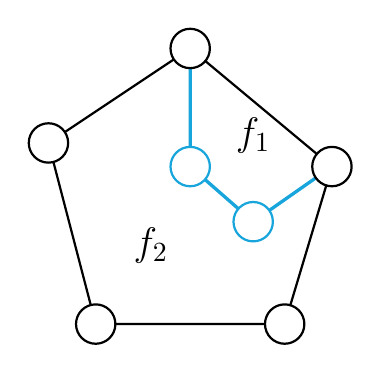
\begin{tikzpicture}[scale=1, auto, swap]
        % ================= 样式定义 =================
        \tikzset{
            % 节点:标准白底黑边
            vnode/.style={circle, draw=black, thick, fill=white, minimum size=5mm, inner sep=0pt},
            % 外部圈边:黑色加粗
            edge/.style={thick, black},
            % 耳朵边:青蓝色加粗
            ear/.style={very thick, cyan!90!black}
        }

        % ================= 1. 定义顶点坐标 =================
        
        % --- 外部圈的 5 个顶点 ---
        \coordinate (n1) at (0, 2);      % Top (连接点1)
        \coordinate (n2) at (-1.8, 0.8); % Left
        \coordinate (n3) at (-1.2, -1.5);% Bottom Left
        \coordinate (n4) at (1.2, -1.5); % Bottom Right
        \coordinate (n5) at (1.8, 0.5);  % Right (连接点2)

        % --- 内部耳的 2 个顶点 ---
        \coordinate (i1) at (0, 0.5);    % Inner 1 (靠上)
        \coordinate (i2) at (0.8, -0.2); % Inner 2 (靠右)

        % ================= 2. 绘制边 =================
        
        % 绘制外部黑色圈
        \draw[edge] (n1) -- (n2) -- (n3) -- (n4) -- (n5) -- (n1);

        % 绘制内部蓝色耳 (路径:Top -> i1 -> i2 -> Right)
        \draw[ear] (n1) -- (i1) -- (i2) -- (n5);

        % ================= 3. 绘制节点 =================
        % 注意:最后画节点以覆盖线头
        
        % 外部节点
        \foreach \p in {n1,n2,n3,n4,n5} \node[vnode] at (\p) {};
        
        % 内部节点 (根据原图,可以使用蓝色边框强调,也可以保持黑色,这里用蓝色边框匹配线条)
        \node[vnode, draw=cyan!90!black] at (i1) {};
        \node[vnode, draw=cyan!90!black] at (i2) {};

        % ================= 4. 标注面 =================
        % f1: 在耳和右上边界围成的区域
        \node at (0.8, 0.9) {\Large $f_1$};
        
        % f2: 在剩余的主区域
        \node at (-0.5, -0.5) {\Large $f_2$};

    \end{tikzpicture}
    \caption{如图演示了在一个圈(黑色边)内加耳(蓝色边)的过程(其实也可以画为圈外,实质等价),分成了两个部分}
\end{figure}

因此,我们就证明了对于 2-连通平面图 $G$ 的任何一种画法,它的任何一个面的边界一定是一个圈,即可以用一个点不重复的回路来遍历。

这个性质证明不难,但非常重要,因为 3-连通图去掉了一个点就是 2-连通图,这很大程度上就是我们为什么要归约到 3-连通图。

\section{收缩引理}

先声明一下,这一部分我们不会涉及有关平面图,画法和交叉的知识,而是全先证明一个对我们后续归纳法至关重要的定理。

首先我们引入收缩操作,形式化而言,对于一个图 $G$ 和其上的任意一条边 $e$ ,我们定义 $G\cdot e$ 为一个新图,如果 $e$ 连接了两个顶点 $\{x,y\}$ ,那么在新图中,这两个顶点将会被合并,而且,这两个顶点的内部连边将会被去掉,从其他顶点连向这两个顶点的边将会连向这个新的顶点。

\begin{figure}[H]
    \centering
    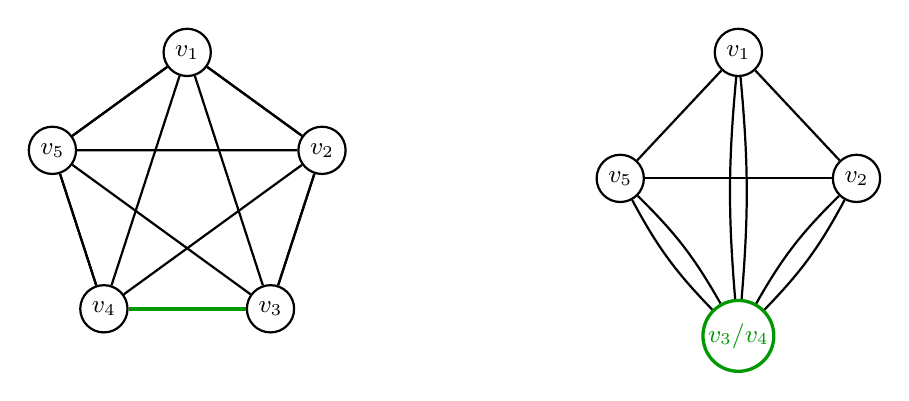
\begin{tikzpicture}[scale=1, auto, swap]
        % ================= 样式定义 =================
        \tikzset{
            % 普通节点
            vnode/.style={circle, draw=black, thick, fill=white, minimum size=6mm, inner sep=0pt, font=\small},
            % 合并后的特殊节点 (稍大,绿色)
            mergednode/.style={circle, draw=green!60!black, very thick, fill=white, minimum size=9mm, inner sep=0pt, font=\small, text=green!60!black},
            % 普通边
            edge/.style={thick, black},
            % 绿色强调边
            green_edge/.style={ultra thick, green!60!black}
        }

        % ================= 左图:K5 (收缩前) =================
        \begin{scope}[shift={(-3.5,0)}]
            % 顶点坐标 (正五边形)
            \node[vnode] (v1) at (90:1.8) {$v_1$};
            \node[vnode] (v5) at (162:1.8) {$v_5$};
            \node[vnode] (v4) at (234:1.8) {$v_4$};
            \node[vnode] (v3) at (306:1.8) {$v_3$};
            \node[vnode] (v2) at (18:1.8) {$v_2$};

            % 绘制普通内部连接
            \draw[edge] (v1)--(v2) (v1)--(v5) (v1)--(v3) (v1)--(v4);
            \draw[edge] (v2)--(v5) (v2)--(v3) (v2)--(v4);
            \draw[edge] (v5)--(v3) (v5)--(v4);
            
            % 绘制外圈 (除了底部那条)
            \draw[edge] (v1)--(v5);
            \draw[edge] (v5)--(v4);
            \draw[edge] (v3)--(v2);
            \draw[edge] (v2)--(v1);

            % 【关键】待收缩的边 v3-v4 (绿色)
            \draw[green_edge] (v4) -- (v3);
        \end{scope}

        % ================= 右图:收缩后 (Contracted) =================
        \begin{scope}[shift={(3.5,0)}]
            % 顶点坐标
            \node[vnode] (u1) at (0, 1.8) {$v_1$};
            \node[vnode] (u5) at (-1.5, 0.2) {$v_5$};
            \node[vnode] (u2) at (1.5, 0.2) {$v_2$};
            
            % 合并后的节点 (位于底部)
            \node[mergednode] (u34) at (0, -1.8) {$v_3/v_4$};

            % 1. 上半部分的普通连接 (保留)
            \draw[edge] (u1) -- (u5);
            \draw[edge] (u1) -- (u2);
            \draw[edge] (u5) -- (u2); % 横梁

            % 2. 通向合并点的重边 (Double Edges)
            % 原图中 v1, v5, v2 都通过两根线连向合并点
            
            % v1 -> v3/v4 (中间垂直的双线)
            \draw[edge] (u1) to[bend right=5] (u34);
            \draw[edge] (u1) to[bend left=5] (u34);

            % v5 -> v3/v4 (左侧的双线)
            \draw[edge] (u5) to[bend right=8] (u34);
            \draw[edge] (u5) to[bend left=8] (u34);

            % v2 -> v3/v4 (右侧的双线)
            \draw[edge] (u2) to[bend right=8] (u34);
            \draw[edge] (u2) to[bend left=8] (u34);

        \end{scope}

    \end{tikzpicture}
    \caption{如图展示了对 $K_5$ 的一条边($v_3-v_4$)进行缩边操作的结果}
\end{figure}

那么既然缩边这个操作那么重要,那么对于一个 3-连通的图 $G$ ,对其任意一条边 $e$ ,缩边后得到的图 $G\cdot e$ 是否仍然是 3-连通呢?这是错误的!一个典型的例子就是下面的轮图,如果对其中心点连接的任意一条辐条边进行缩边,图便会由 3-连通变为 2-连通:

\begin{figure}[H]
    \centering
    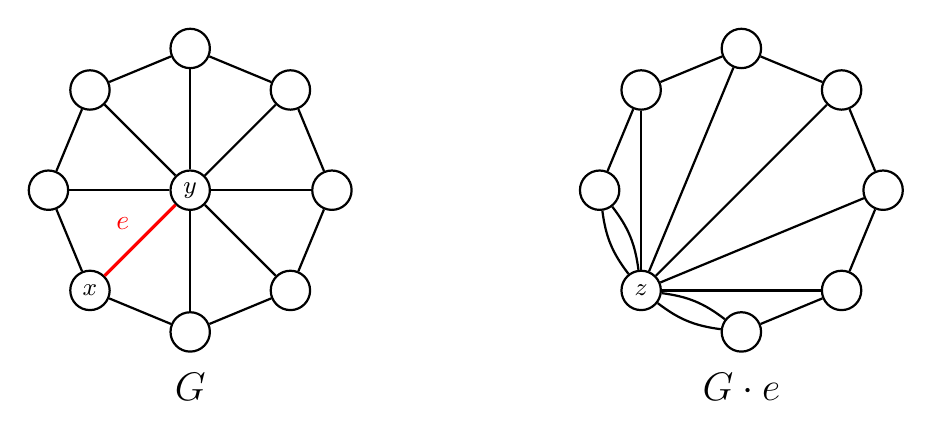
\begin{tikzpicture}[scale=1, auto, swap]
        % ================= 样式定义 =================
        \tikzset{
            vnode/.style={circle, draw=black, thick, fill=white, minimum size=5mm, inner sep=0pt, font=\small},
            edge/.style={thick, black},
            red_edge/.style={very thick, red}
        }

        % ================= 左图:G (轮图) =================
        \begin{scope}[shift={(-3.5,0)}]
            % 1. 中心点 y
            \node[vnode] (y) at (0,0) {$y$};

            % 2. 外圈点 (8个)
            % x 在 225 度 (节点 n4)
            % 邻居是 n3 (180度) 和 n5 (270度)
            \foreach \i/\angle in {1/90, 2/135, 3/180, 4/225, 5/270, 6/315, 7/0, 8/45} {
                \ifnum\i=4
                    \node[vnode] (n\i) at (\angle:1.8) {$x$};
                \else
                    \node[vnode] (n\i) at (\angle:1.8) {};
                \fi
            }

            % 3. 绘制外圈连边
            \draw[edge] (n1)--(n2)--(n3)--(n4)--(n5)--(n6)--(n7)--(n8)--(n1);

            % 4. 绘制辐条
            \foreach \i in {1,2,3,5,6,7,8} {
                \draw[edge] (y) -- (n\i);
            }

            % 5. 红色缩边
            \draw[red_edge] (n4) -- node[above left, text=red] {$e$} (y);
            
            \node at (0, -2.5) {\Large $G$};
        \end{scope}

        % ================= 右图:G.e (突出重边) =================
        \begin{scope}[shift={(3.5,0)}]
            
            % 1. 绘制原本外圈的点 (除了 x)
            % u3 和 u5 是关键邻居
            \foreach \i/\angle in {1/90, 2/135, 3/180, 5/270, 6/315, 7/0, 8/45} {
                \node[vnode] (u\i) at (\angle:1.8) {};
            }
            
            % 2. 绘制合并点 z (在原本 x 的位置)
            \node[vnode] (z) at (225:1.8) {$z$};

            % 3. 绘制外圈剩余部分的单边 (Chain)
            % 从 u5 -> u6 ... -> u1 -> u2 -> u3
            \draw[edge] (u5)--(u6)--(u7)--(u8)--(u1)--(u2)--(u3);

            % 4. 绘制原本的辐条 (单边)
            % 这些点原本只和 y 连,不和 x 连,所以合并后只有一条边
            \foreach \i in {1,2,6,7,8} {
                \draw[edge] (z) -- (u\i);
            }

            % 5. 【关键】绘制重边 (Double Edges)
            % z 连接 u3 (左邻居) 和 u5 (下邻居)
            % 原理:一条来自原本的轮廓边,一条来自原本的辐条边
            
            % z <-> u3 的重边
            \draw[edge] (z) to[bend right=15] (u3);
            \draw[edge] (z) to[bend left=15] (u3);

            % z <-> u5 的重边
            \draw[edge] (z) to[bend right=15] (u5);
            \draw[edge] (z) to[bend left=15] (u5);
            
            \node at (0, -2.5) {\Large $G \cdot e$};
        \end{scope}

    \end{tikzpicture}
    \caption{如图,红色边 $e$ 是左图中被缩的边,缩边原本的 $x,y$ 合并成点 $z$,右图中,删掉 $z$ 得到一条链,注意 $z$ 与其邻居形成了重边}
\end{figure}

这就是为什么我们要大费周章并谨慎地证明下面这个更弱但够用的结论。即,对于一个顶点数 $n\ge 5$ 的 3-连通图 $G$ ,一定存在一条边 $e$ ,使得缩边后的结果 $G\cdot e$ 是 3-连通图。

我们采用反证法论证这个命题的正确性。

这里之所以强制让顶点数不小于 5,是为了让图 3-连通这个条件,严格等价于存在一个删去三个顶点的方法使得图出现至少两个连通分支,后续我们将不再强调点数的作用,但这里特此说明。

\subsection{反证分析}
假设这个命题是错的,那么一定存在一个 3-连通图 $G$ ,满足对于任意 $e\in G$ 都有 $G\cdot e$ 不是 3-连通的。

好的,我们考虑对于一个图 $G$ ,对 $e$ 进行缩边后, $G\cdot e$ 存在两个顶点的点割集 $\{u,z\}$ 使得图不连通,我们断言一定有一个顶点是新出现的合并点,这是因为如果 $u,z$ 都是原有的点,那么我们直接把缩边操作撤回,再删去点,连通分量的个数是不变的(具体而言,可以证明 $e$ 的两端由于互相可达,它们到达的点并不会因此发生改变);这就意味着 $\{u,z\}$ 也可以成为原图 $G$ 的点割集,矛盾。

因此不妨设 $u$ 是新出现的合并点,它合并了原图 $G$ 中的 $x,y$ 两个顶点( $e$ 的两个端点是 $x,y$ ),那么就有 $\{x,y,z\}$ 是原图 $G$ 的点割集了。

好的,那么我们的意思是,如果这样的图 $G$ 存在,那么对于 $G$ 的任意一条边 $e$ 的两个端点 $x,y$ ,总存在一个顶点 $z$ 使得删掉 $x,y,z$ 之后图不连通,就好像每条边都有一个伴侣。

\subsection{寻找最大的更大}
那么不妨定义对于 $G$ 上的满足条件的 $e,z$ ,定义这种选取的价值为删去 $e$ 的两个端点 $x,y$ 和顶点 $z$ 后形成的若干连通分量中最大的连通分量的大小。

既然选取方案数量有限,那么我们找到价值最大的一种方案,不妨设为 $e,z$ ,其中 $e$ 的端点为 $x,y$ ,那么删去 $x,y,z$ 三个顶点后会形成至少两个连通分量,不妨设最大的为 $G_1$ ,从剩下的连通分量任取一个为 $G_2$ 。

那么由于图是 3-连通的,所以 $x,y,z$ 必然和 $G_1,G_2$ 各自都有连边。

\begin{figure}[H]
    \centering
    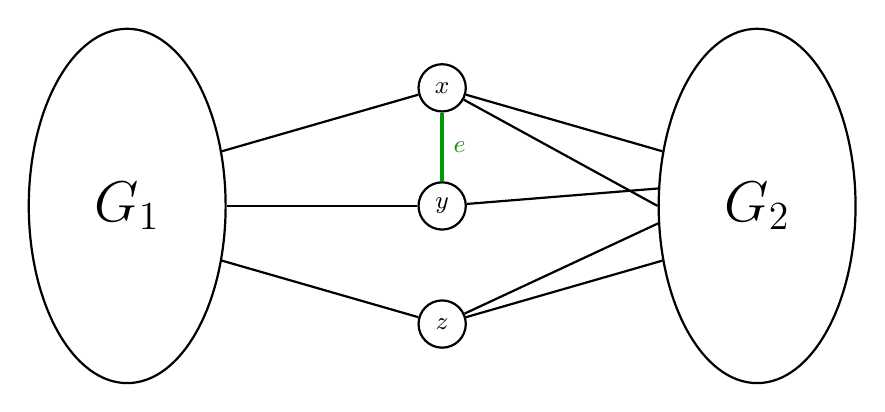
\begin{tikzpicture}[scale=1, auto, swap]
        % ================= 样式定义 =================
        \tikzset{
            % 连通分量样式:大椭圆
            blob/.style={draw=black, thick, fill=white, align=center, font=\huge, minimum width=2.5cm, minimum height=4.5cm},
            % 割集顶点样式
            vnode/.style={circle, draw=black, thick, fill=white, minimum size=6mm, inner sep=0pt, font=\small},
            % 普通连边
            edge/.style={thick, black},
            % 缩边 e 的特殊颜色
            contract_edge/.style={ultra thick, green!60!black}
        }

        % ================= 1. 绘制左侧 G1 和右侧 G2 =================
        \node[blob, ellipse] (G1) at (-4, 0) {$G_1$};
        \node[blob, ellipse] (G2) at (4, 0) {$G_2$};

        % ================= 2. 绘制中间割集 {x, y, z} =================
        \node[vnode] (x) at (0, 1.5) {$x$};
        \node[vnode] (y) at (0, 0) {$y$};
        \node[vnode] (z) at (0, -1.5) {$z$};

        % ================= 3. 绘制边 =================

        % --- 缩边 e (x-y) ---
        \draw[contract_edge] (x) -- node[right, font=\small, text=green!60!black] {$e$} (y);

        % --- x, y, z 到 G1 的连边 ---
        \draw[edge] (x) -- (G1.30);
        \draw[edge] (y) -- (G1.0);
        \draw[edge] (z) -- (G1.330);

        % --- x, y, z 到 G2 的连边 ---
        % 注意这里按照你的原图,x 到 G2 有两条,y 有一条,z 有两条
        \draw[edge] (x) -- (G2.150);
        \draw[edge] (x) -- (G2.180); % 对应原图交叉的那根
        \draw[edge] (y) -- (G2.170); 
        \draw[edge] (z) -- (G2.190);
        \draw[edge] (z) -- (G2.210);

    \end{tikzpicture}
    \caption{如图所示,其中 $e$ 是连接 $x,y$ 的边,$x,y,z$ 分别和 $G_1$ $G_2$ 各有至少一条连边}
\end{figure}

那么,任取 $z$ 在 $G_2$ 的一个邻居 $u$ ,由于 $z,u$ 是 $G$ 上一条边的两个端点,由反证假设,必存在顶点 $v$ 使得 $G$ 删去 $\{z,u,v\}$ 不连通。

那么我们考察这次选取的价值,即删去 $\{z,u,v\}$ 之后连通分量最大的是多少。

\subsection{证明更大并导出矛盾}
如果我们能证明 $G$ 删去 $\{z,u,v\}$ 之后 $G_1$ 的所有顶点的导出子图仍然连通,那么我们就可能证明这次选取的价值更大。

具体而言,设 $H=G_1\cup \{x,y\}$ ,它的导出子图在 $G$ 中一定连通,注意到 $z,u$ 一定都不属于 $H$ ,而 $v$ 的情况不确定。

首先如果 $v\notin H$ 那么 $H$ 内的顶点的导出子图连通性保持,且比 $G_1$ 多两个顶点,那显然 $\{z,u,v\}$ 价值更大。

如果 $v\in H$ 且删去 $v$ 仍然使得 $H$ 内的其它顶点的导出子图连通,那么 $H-\{v\}$ 仍然比 $G_1$ 多一个顶点, $\{z,u,v\}$ 价值仍然更大。

显然 $v=x$ 或 $v=y$ 不会影响 $H$ 的导出子图的连通性,考虑 $v\in G_1$ 会不会影响。

\begin{figure}[H]
    \centering
    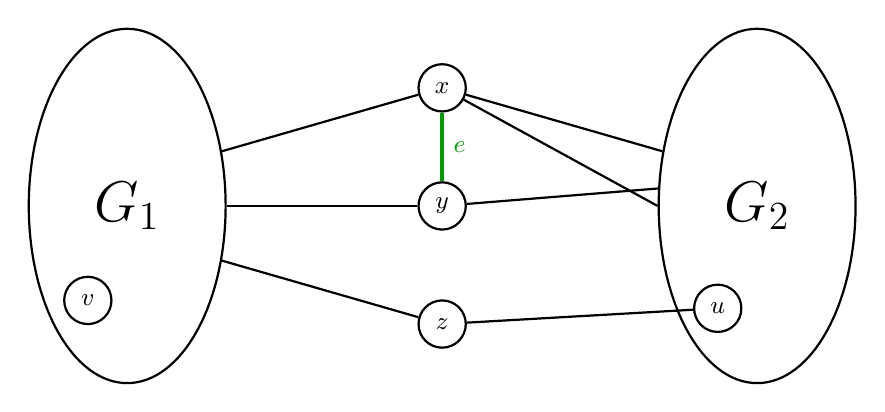
\begin{tikzpicture}[scale=1, auto, swap]
        % ================= 样式定义 (保持一致) =================
        \tikzset{
            % 连通分量样式:大椭圆
            blob/.style={draw=black, thick, fill=white, align=center, font=\huge, minimum width=2.5cm, minimum height=4.5cm},
            % 普通顶点样式
            vnode/.style={circle, draw=black, thick, fill=white, minimum size=6mm, inner sep=0pt, font=\small},
            % 普通连边
            edge/.style={thick, black},
            % 缩边 e 的特殊颜色
            contract_edge/.style={ultra thick, green!60!black}
        }

        % ================= 1. 绘制大椭圆 G1 和 G2 =================
        \node[blob, ellipse] (G1) at (-4, 0) {$G_1$};
        \node[blob, ellipse] (G2) at (4, 0) {$G_2$};

        % ================= 2. 绘制中间割集 {x, y, z} =================
        \node[vnode] (x) at (0, 1.5) {$x$};
        \node[vnode] (y) at (0, 0) {$y$};
        \node[vnode] (z) at (0, -1.5) {$z$};

        % ================= 3. 【新增】绘制内部点 v 和 u =================
        % v 在 G1 内部左下放
        \node[vnode] (v) at (-4.5, -1.2) {$v$};
        % u 在 G2 内部左下放,靠近 z 的连接处
        \node[vnode] (u) at (3.5, -1.3) {$u$};

        % ================= 4. 绘制边 =================

        % --- 缩边 e (x-y) ---
        \draw[contract_edge] (x) -- node[right, font=\small, text=green!60!black] {$e$} (y);

        % --- x, y, z 到 G1 的连边 (连向边界) ---
        \draw[edge] (x) -- (G1.30);
        \draw[edge] (y) -- (G1.0);
        \draw[edge] (z) -- (G1.330);

        % --- x, y 到 G2 的连边 (连向边界) ---
        \draw[edge] (x) -- (G2.150);
        \draw[edge] (x) -- (G2.180); % 交叉的那根
        \draw[edge] (y) -- (G2.170);

        % --- 【修改】z 到 G2 的连边 (现在连向内部的 u) ---
        \draw[edge] (z) -- (u);

    \end{tikzpicture}
    \caption{如图所示,如果 $v$ 属于 $G_1$,会不会影响 $H$ 内导出子图的连通性呢?}
\end{figure}

先删去 $v$ ,假设 $H$ 的导出子图因为 $v$ 被删掉分割成了多个连通分量,由于 $x,y$ 之间的直连边不受影响,它们必然在同一个连通分支,既然 $H-\{v\}$ 的导出子图不连通,考虑取出 $H-\{v\}$ 中不和 $x,y$ 在同一个连通分量的分量 $H_1$ ,显然为了让 $v$ 不是 $G$ 的割点(否则会破坏 3-连通性),必须让 $H_1$ 与 $z$ 相连,但即使如此,删去 $z$ 之后, $H_1$ 也会形成一个单独的连通分量,也就是 $G-\{z,v\}$ 不连通,这同样与 $G$ 的 3-连通性矛盾。

\begin{figure}[H]
    \centering
    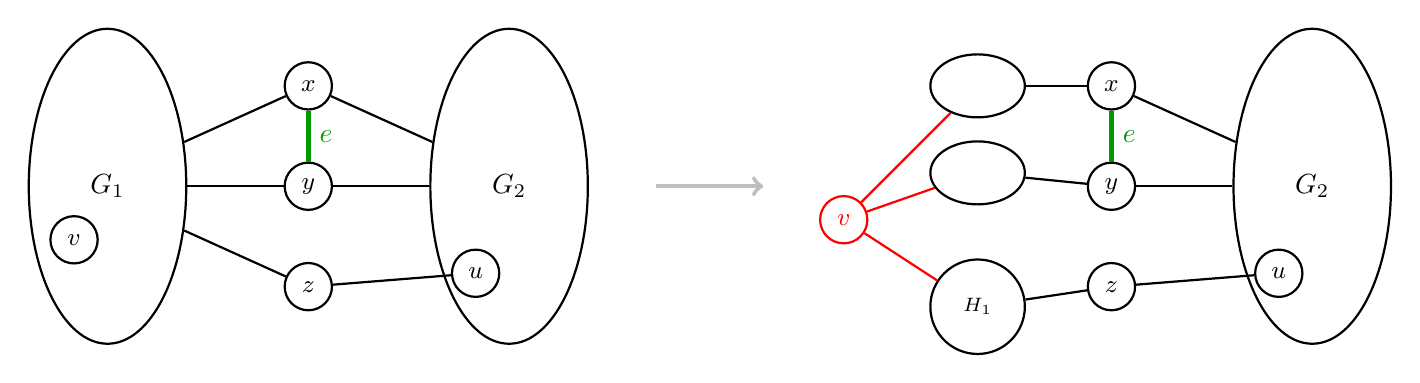
\begin{tikzpicture}[scale=0.85, auto, swap]
        % ================= 样式定义 =================
        \tikzset{
            % 大连通块
            blob/.style={draw=black, thick, fill=white, align=center, ellipse, minimum width=2cm, minimum height=4cm},
            % 小连通块 (H 的分量)
            subblob/.style={draw=black, thick, fill=white, align=center, ellipse, minimum width=1.2cm, minimum height=0.8cm, font=\scriptsize},
            % 顶点
            vnode/.style={circle, draw=black, thick, fill=white, minimum size=6mm, inner sep=0pt, font=\small},
            % 强调顶点 (红色)
            rednode/.style={circle, draw=red, thick, fill=white, minimum size=6mm, inner sep=0pt, font=\small, text=red},
            % 普通边
            edge/.style={thick, black},
            % 缩边 e
            contract_edge/.style={ultra thick, green!60!black},
            % 矛盾边 (红色)
            red_edge/.style={thick, red}
        }

        % ================= 左侧部分:回顾图 15 (原状态) =================
        \begin{scope}[shift={(-6, 0)}]
            \node[blob] (G1L) at (-3, 0) {$G_1$};
            \node[blob] (G2L) at (3, 0) {$G_2$};
            
            \node[vnode] (xL) at (0, 1.5) {$x$};
            \node[vnode] (yL) at (0, 0) {$y$};
            \node[vnode] (zL) at (0, -1.5) {$z$};
            
            \node[vnode] (vL) at (-3.5, -0.8) {$v$};
            \node[vnode] (uL) at (2.5, -1.3) {$u$};
            
            \draw[contract_edge] (xL) -- (yL) node[midway, right, text=green!60!black] {$e$};
            \draw[edge] (xL) -- (G1L.30); \draw[edge] (xL) -- (G2L.150);
            \draw[edge] (yL) -- (G1L.0); \draw[edge] (yL) -- (G2L.180);
            \draw[edge] (zL) -- (G1L.330); \draw[edge] (zL) -- (uL);
        \end{scope}

        % ================= 右侧部分:展示 G1 的分解 (证明逻辑) =================
        \begin{scope}[shift={(6, 0)}]
            % 绘制右侧保持不变的 G2
            \node[blob] (G2R) at (3, 0) {$G_2$};
            \node[vnode] (uR) at (2.5, -1.3) {$u$};
            
            % 绘制中间割集
            \node[vnode] (xR) at (0, 1.5) {$x$};
            \node[vnode] (yR) at (0, 0) {$y$};
            \node[vnode] (zR) at (0, -1.5) {$z$};
            
            % 绘制 G1 分解后的三个子块 (H 分量)
            \node[subblob] (H_top) at (-2, 1.5) {};
            \node[subblob] (H_mid) at (-2, 0.2) {};
            \node[subblob, minimum height=1.2cm] (H1) at (-2, -1.8) {$H_1$};
            
            % 绘制关键点 v (红色强调)
            \node[rednode] (vR) at (-4, -0.5) {$v$};
            
            % 连接关系
            \draw[contract_edge] (xR) -- (yR) node[midway, right, text=green!60!black] {$e$};
            
            % v 与各分量的红边 (展示 v 是它们的公共邻居)
            \draw[red_edge] (vR) -- (H_top);
            \draw[red_edge] (vR) -- (H_mid);
            \draw[red_edge] (vR) -- (H1);
            
            % x, y, z 与各分量的连接 (展示 H1 的孤立性)
            \draw[edge] (xR) -- (H_top);
            \draw[edge] (yR) -- (H_mid);
            \draw[edge] (zR) -- (H1); % H1 与 z 相连以保证非平凡
            
            % 与 G2 的连接保持
            \draw[edge] (xR) -- (G2R.150);
            \draw[edge] (yR) -- (G2R.180);
            \draw[edge] (zR) -- (uR);
        \end{scope}

        % 画一个中间的箭头表示推导过程 (可选)
        \draw[->, ultra thick, gray!50] (-0.8, 0) -- (0.8, 0);

    \end{tikzpicture}
    \caption{如图所示,可以直观地看到,如果删去 $v$ 使得 $H$ 所在的导出子图不再连通,一定会存在连通分量 $H_1$,它可以证明删去 $v,z$ 之后整个子图是不连通的,这破坏了 $G$ 的 3-连通性}
\end{figure}

因此不论如何,删去 $\{z,u,v\}$ 总是会使得剩余的连通分支包含 $H$ 的大部分,即使 $v\in H$ ,仍然存在连通分支至少比 $G_1$ 要大一。即证明了对于任意边点选取,总存在价值严格更大的边点选取,这是完全不可能的,因为对于有限图,边点选取的总数是有限的。

因此,只剩下一种可能,那就是反证法假设的基础,存在一个 3-连通图 $G$ ,满足对于任意 $e\in G$ 都有 $G\cdot e$ 不是 3-连通的,这一命题是不成立的。

因此我们就证明了,对于一个顶点数 $n\ge 5$ 的 3-连通图 $G$ ,一定存在一条边 $e$ ,使得缩边后的结果 $G\cdot e$ 是 3-连通图。

那么你可能会感觉这一部分好像和平面图一点关系也没有啊,是这样的,之所以扯了这一节完全是为了证明收缩引理,接下来我们还要证明一个收缩性质,这次,和平面图沾了一点边。

\section{收缩的性质}
这个性质不依赖 $G$ 的 3-连通性。

收缩操作有一个特殊的性质,那就是,如果一个图 $G$ 不含有 $K_{5}$ 或 $K_{3,3}$ 的细分作为子图;那么 $G\cdot e$ 一定不含 $K_{5}$ 或 $K_{3,3}$ 的细分作为子图。

那么,这等价于证明,如果 $G\cdot e$ 含有 $K_{5}$ 或 $K_{3,3}$ 的细分作为子图,那么 $G$ 一定含有 $K_{5}$ 或 $K_{3,3}$ 的细分作为子图。

不妨设 $G\cdot e$ 将原本 $G$ 中的 $x,y$ 两个顶点收缩成了顶点 $z$ 。

首先如果 $z$ 不属于某个 $G\cdot e$ 的 $K_{5}$ 或 $K_{3,3}$ 的细分子图,那么显然,这个子图在 $G$ 中原样存在,那么 $G$ 含有 $K_{5}$ 或 $K_{3,3}$ 的细分作为子图。

其次 $z$ 属于某个 $G\cdot e$ 的 $K_{5}$ 或 $K_{3,3}$ 的细分子图,且在这个细分子图内度数为 2(也就是细分路径上的一个顶点),那么显然,这个细分子图在 $G$ 中也是 $K_{5}$ 或 $K_{3,3}$ 的细分,只不过某条路径拉长了一点,那么 $G$ 仍然含有 $K_{5}$ 或 $K_{3,3}$ 的细分作为子图。

\begin{figure}[H]
    \centering
    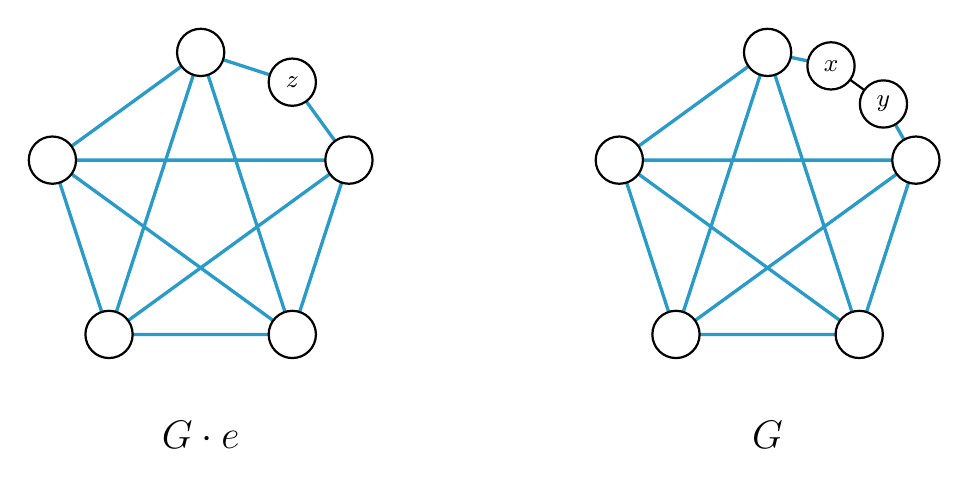
\begin{tikzpicture}[scale=0.9, auto, swap]
        % ================= 样式定义 (完全参照你的标准模板) =================
        \tikzset{
            % 节点样式:白底黑边圆圈
            vnode/.style={circle, draw=black, thick, fill=white, minimum size=6mm, inner sep=0pt, font=\small},
            % 蓝色路径样式 (代表细分路径)
            blue_path/.style={very thick, cyan!80!black},
            % 黑色收缩边样式
            contract_edge/.style={thick, black}
        }

        % ================= 左图:G.e (z 是度数为 2 的细分点) =================
        \begin{scope}[shift={(-4,0)}]
            % 1. 定义 5 个支点的位置
            \foreach \i in {1,...,5} {
                \coordinate (p\i) at (90 - 72*\i + 72:2.2);
            }

            % 2. 绘制基础蓝边 (除 p1-p2 以外的所有 K5 边)
            % 内部星形
            \draw[blue_path] (p1)--(p3) (p1)--(p4) (p2)--(p4) (p2)--(p5) (p3)--(p5);
            % 外部五边形 (跳过 p1-p2)
            \draw[blue_path] (p2)--(p3) (p3)--(p4) (p4)--(p5) (p5)--(p1);

            % 3. 绘制 z 及其所在的细分路径
            \coordinate (z_pos) at (54:2.2); % 位于 p1 和 p2 之间
            \draw[blue_path] (p1) -- (z_pos) -- (p2);

            % 4. 放置节点
            \foreach \i in {1,...,5} \node[vnode] at (p\i) {};
            \node[vnode] (z) at (z_pos) {$z$};

            \node at (0, -3.2) {\Large $G \cdot e$};
        \end{scope}

        % ================= 右图:G (z 拆分为 x-y,路径变长) =================
        \begin{scope}[shift={(4,0)}]
            % 1. 定义 5 个支点的位置
            \foreach \i in {1,...,5} {
                \coordinate (q\i) at (90 - 72*\i + 72:2.2);
            }

            % 2. 绘制基础蓝边
            \draw[blue_path] (q1)--(q3) (q1)--(q4) (q2)--(q4) (q2)--(q5) (q3)--(q5);
            \draw[blue_path] (q2)--(q3) (q3)--(q4) (q4)--(q5) (q5)--(q1);

            % 3. 在 q1-q2 之间插入 x, y 以及黑色的边 e
            \coordinate (x_pos) at (66:2.2);
            \coordinate (y_pos) at (42:2.2);
            
            \draw[blue_path] (q1) -- (x_pos);
            \draw[blue_path] (y_pos) -- (q2);
            \draw[contract_edge] (x_pos) -- node[right, font=\scriptsize] {} (y_pos);

            % 4. 放置节点
            \foreach \i in {1,...,5} \node[vnode] at (q\i) {};
            \node[vnode] (x) at (x_pos) {$x$};
            \node[vnode] (y) at (y_pos) {$y$};

            \node at (0, -3.2) {\Large $G$};
        \end{scope}

    \end{tikzpicture}
    \caption{如图是 $K_5$ 上,$z$ 是子图上度数为 2 的点,其中蓝色线代表路径,黑色线代表边,显然,收缩后存在 $K_5$ 细分,收缩前仍然存在,只不过某条路径更长一点}
\end{figure}

剩下的情况是, $z$ 属于某个 $G\cdot e$ 的 $K_{5}$ 或 $K_{3,3}$ 的细分子图,且在这个细分子图内度数为 3( $K_{3,3}$ 上的分支顶点)或 4( $K_5$ 上的分支顶点)。

\subsection{收缩后度数为 3}
那么 $z$ 度数(在 $G\cdot e$ 的细分子图上,后同)为 3,是 $K_{3,3}$ 上的分支顶点,考虑原图 $x,y$ 的情况,不妨设 $x$ 的度数不大于 $y$ ,那么有两种情况:

1. $x$ 在忽略到 $y$ 的连边后,向其它地方延伸出 0 条边; $y$ 在忽略到 $x$ 的连边后,向其它地方延伸出 3 条边,此时直接把 $y$ 当作 $z$ 即可, $G$ 中存在 $K_{3,3}$ 的细分。

\begin{figure}[H]
    \centering
    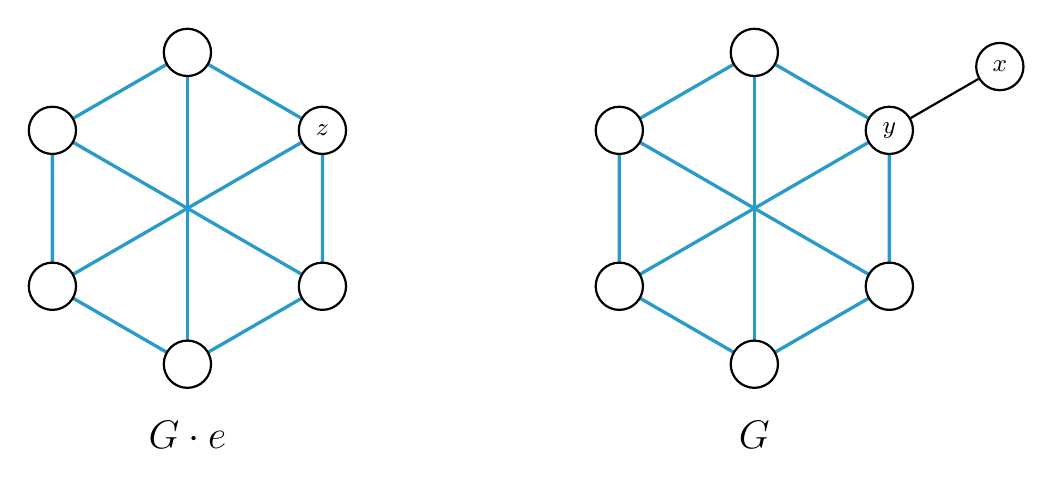
\begin{tikzpicture}[scale=0.9, auto, swap]
        % ================= 样式定义 (完全参照你的标准模板) =================
        \tikzset{
            % 节点样式:白底黑边圆圈
            vnode/.style={circle, draw=black, thick, fill=white, minimum size=6mm, inner sep=0pt, font=\small},
            % 蓝色路径样式 (代表细分路径)
            blue_path/.style={very thick, cyan!80!black},
            % 黑色收缩边样式
            contract_edge/.style={thick, black}
        }

        % ================= 左图:G.e (K3,3 收缩图) =================
        \begin{scope}[shift={(-4,0)}]
            % 定义 6 个顶点的位置 (对称六边形布局)
            \foreach \i in {1,...,6} {
                \coordinate (p\i) at (150 - 60*\i + 60:2.2);
            }

            % 绘制 K3,3 的边 (外圈 6 条 + 对角线 3 条)
            \draw[blue_path] (p1) -- (p2) -- (p3) -- (p4) -- (p5) -- (p6) -- (p1);
            \foreach \i in {1,2,3} {
                \pgfmathtruncatemacro{\j}{\i+3}
                \draw[blue_path] (p\i) -- (p\j);
            }

            % 绘制节点,将右上角的节点标记为 z (对应 p3)
            \foreach \i in {1,2,4,5,6} \node[vnode] at (p\i) {};
            \node[vnode] (z) at (p3) {$z$}; 

            \node at (0, -3.2) {\Large $G \cdot e$};
        \end{scope}

        % ================= 右图:G (x 作为叶子) =================
        \begin{scope}[shift={(4,0)}]
            % 6 个基本顶点位置
            \foreach \i in {1,...,6} {
                \coordinate (q\i) at (150 - 60*\i + 60:2.2);
            }

            % 绘制骨架 (y 继承 z 的位置)
            \draw[blue_path] (q1) -- (q2) -- (q3) -- (q4) -- (q5) -- (q6) -- (q1);
            \foreach \i in {1,2,3} {
                \pgfmathtruncatemacro{\j}{\i+3}
                \draw[blue_path] (q\i) -- (q\j);
            }

            \foreach \i in {1,2,4,5,6} \node[vnode] at (q\i) {};
            \node[vnode] (y) at (q3) {$y$};
            
            % x 作为叶子节点,按照 image_1fd718.png 所示向斜上方(55度)延伸,不干扰骨架
            \node[vnode] (x) at (30:4) {$x$};
            
            % 绘制黑色的待收缩边 e
            \draw[contract_edge] (x) -- node[right, font=\scriptsize] {} (y);

            \node at (0, -3.2) {\Large $G$};
        \end{scope}

    \end{tikzpicture}
    \caption{如图是 $K_{3,3}$ 的情况,左图是细分之后,右图是未细分,蓝色是路径,黑色是边,如果 $x$ 可以作为叶子,不管即可,此时 $G$ 中有 $K_{3,3}$ 的细分}
\end{figure}

2. $x$ 在忽略到 $y$ 的连边后,向其它地方延伸出 1 条边; $y$ 在忽略到 $x$ 的连边后,向其它地方延伸出 2 条边,此时直接把 $y$ 当作 $z$ ,且 $x$ 当作 $y$ 延伸的 3 条路径中的其中一条路径上的细分。

\begin{figure}[H]
    \centering
    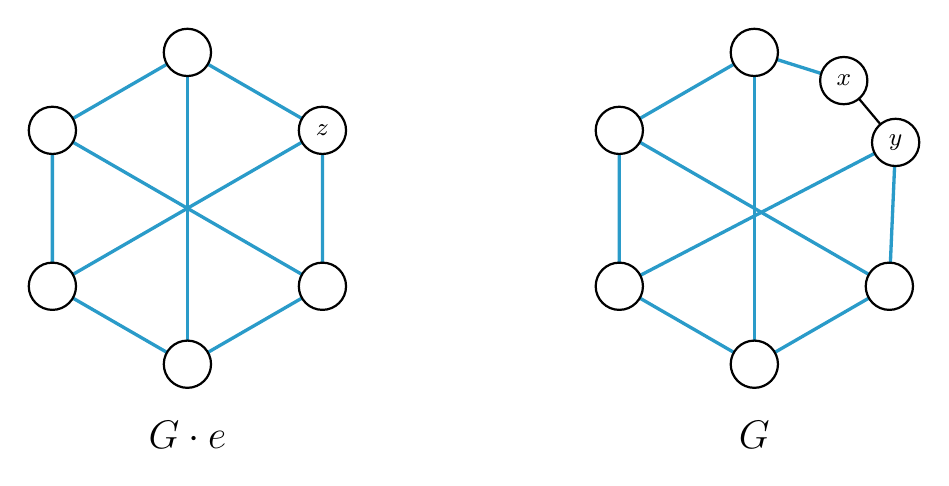
\begin{tikzpicture}[scale=0.9, auto, swap]
        % ================= 样式定义 (完全参照你的标准模板) =================
        \tikzset{
            % 节点样式:白底黑边圆圈
            vnode/.style={circle, draw=black, thick, fill=white, minimum size=6mm, inner sep=0pt, font=\small},
            % 蓝色路径样式 (代表细分路径)
            blue_path/.style={very thick, cyan!80!black},
            % 黑色收缩边样式
            contract_edge/.style={thick, black}
        }

        % ================= 左图:G.e (z 是度数为 3 的分支顶点) =================
        \begin{scope}[shift={(-4,0)}]
            % 定义 6 个顶点位置 (六边形布局)
            \foreach \i in {1,...,6} {
                \coordinate (p\i) at (150 - 60*\i + 60:2.2);
            }

            % 绘制 K3,3 的边 (外圈 6 条 + 对角线 3 条)
            \draw[blue_path] (p1) -- (p2) -- (p3) -- (p4) -- (p5) -- (p6) -- (p1);
            \draw[blue_path] (p1) -- (p4);
            \draw[blue_path] (p2) -- (p5);
            \draw[blue_path] (p3) -- (p6);

            % 标记 z 为右上角的节点 (p3)
            \foreach \i in {1,2,4,5,6} \node[vnode] at (p\i) {};
            \node[vnode] (z) at (p3) {$z$}; 

            \node at (0, -3.2) {\Large $G \cdot e$};
        \end{scope}

        % ================= 右图:G (x 连 1 条,y 连 2 条) =================
        \begin{scope}[shift={(4,0)}]
            % 定义 5 个骨架顶点位置
            \coordinate (q1) at (150:2.2);
            \coordinate (q2) at (90:2.2);
            \coordinate (q4) at (330:2.2);
            \coordinate (q5) at (270:2.2);
            \coordinate (q6) at (210:2.2);
            
            % 将原本 z 的位置 (30度) 拆分为 y 和 x
            % y 靠近原本的 p4 和 p6 方向,x 靠近 p2 方向
            \coordinate (q3_y) at (25:2.2);
            \coordinate (q3_x) at (55:2.2);

            % 绘制骨架蓝边 (不含与 x, y 相关的部分)
            \draw[blue_path] (q4) -- (q5) -- (q6) -- (q1) -- (q2);
            \draw[blue_path] (q1) -- (q4);
            \draw[blue_path] (q2) -- (q5);

            % 分配邻居:
            % y 连向 q4 (外圈) 和 q6 (对角线) -> 共 2 条
            \draw[blue_path] (q3_y) -- (q4);
            \draw[blue_path] (q3_y) -- (q6);
            % x 连向 q2 (外圈) -> 共 1 条
            \draw[blue_path] (q3_x) -- (q2);

            % 绘制黑色的收缩边 e 连接 x 和 y
            \draw[contract_edge] (q3_x) -- node[right, font=\scriptsize] {} (q3_y);

            % 绘制节点
            \node[vnode] at (q1) {};
            \node[vnode] at (q2) {};
            \node[vnode] at (q4) {};
            \node[vnode] at (q5) {};
            \node[vnode] at (q6) {};
            \node[vnode] (y) at (q3_y) {$y$};
            \node[vnode] (x) at (q3_x) {$x$};

            \node at (0, -3.2) {\Large $G$};
        \end{scope}

    \end{tikzpicture}
    \caption{如图是 $K_{3,3}$ 的情况,左图是细分之后,右图是未细分,蓝色是路径,黑色是边,如果 $x$ 不是叶子,度数较小的点仍然只够做路径上的分支,此时 $G$ 中有 $K_{3,3}$ 的细分}
\end{figure}

因此这两种情况都可以让 $G$ 中存在一个 $K_{3,3}$ 的细分。

\subsection{收缩后度数为 4}
那么 $z$ 度数(在 $G\cdot e$ 的细分子图上,后同)为 4,$K_5$ 上的分支顶点,考虑原图 $x,y$ 的情况,不妨设 $x$ 的度数不大于 $y$ ,那么有三种情况:

1. $x$ 在忽略到 $y$ 的连边后,向其它地方延伸出 0 条边; $y$ 在忽略到 $x$ 的连边后,向其它地方延伸出 4 条边,此时直接把 $y$ 当作 $z$ 即可, $G$ 中存在 $K_5$ 的细分。

\begin{figure}[H]
    \centering
    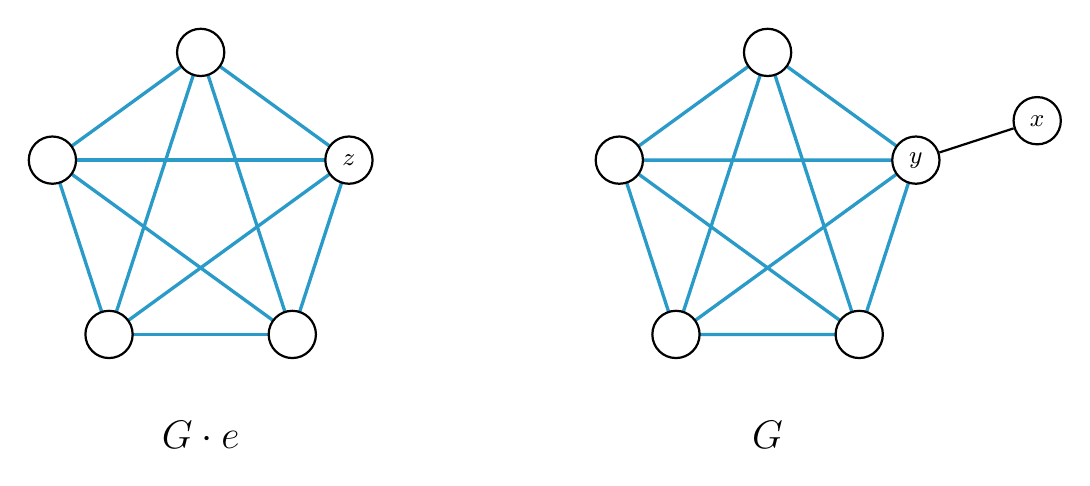
\begin{tikzpicture}[scale=0.9, auto, swap]
        % ================= 样式定义 (保持一致) =================
        \tikzset{
            vnode/.style={circle, draw=black, thick, fill=white, minimum size=6mm, inner sep=0pt, font=\small},
            blue_path/.style={very thick, cyan!80!black},
            contract_edge/.style={thick, black}
        }

        % ================= 左图:G.e (K5 收缩图) =================
        \begin{scope}[shift={(-4,0)}]
            % 定义 5 个顶点位置
            \foreach \i in {1,...,5} {
                \coordinate (p\i) at (90 - 72*\i + 72:2.2);
            }

            % 绘制 K5 的 10 条蓝边
            \foreach \i in {1,...,4} {
                \pgfmathtruncatemacro{\ip}{\i+1}
                \foreach \j in {\ip,...,5} {
                    \draw[blue_path] (p\i) -- (p\j);
                }
            }

            % 绘制节点,将右上角节点标记为 z (p2)
            \foreach \i in {1,3,4,5} \node[vnode] at (p\i) {};
            \node[vnode] (z) at (p2) {$z$}; 

            \node at (0, -3.2) {\Large $G \cdot e$};
        \end{scope}

        % ================= 右图:G (x 作为叶子) =================
        \begin{scope}[shift={(4,0)}]
            % 5 个基本顶点位置
            \foreach \i in {1,...,5} {
                \coordinate (q\i) at (90 - 72*\i + 72:2.2);
            }

            % 绘制 y 及其邻居间的蓝边 (构成完整 K5)
            % 1. 绘制其余 4 个邻居间的 K4
            \draw[blue_path] (q1)--(q3) (q1)--(q4) (q1)--(q5) (q3)--(q4) (q3)--(q5) (q4)--(q5);
            % 2. 绘制 y 与这 4 个邻居的连线
            \draw[blue_path] (q2)--(q1) (q2)--(q3) (q2)--(q4) (q2)--(q5);

            % 绘制节点
            \foreach \i in {1,3,4,5} \node[vnode] at (q\i) {};
            \node[vnode] (y) at (q2) {$y$};
            
            % x 作为叶子节点,向外偏移
            \node[vnode] (x) at (18:4) {$x$};
            
            % 绘制黑色的待收缩边 (不带 e 标注)
            \draw[contract_edge] (x) -- (y);

            \node at (0, -3.2) {\Large $G$};
        \end{scope}

    \end{tikzpicture}
    \caption{如图是 $K_5$ 的情况,左图是细分之后,右图是未细分,蓝色是路径,黑色是边,如果 $x$ 可以作为叶子,不管即可,此时 $G$ 中有 $K_5$ 的细分}
\end{figure}

2. $x$ 在忽略到 $y$ 的连边后,向其它地方延伸出 1 条边; $y$ 在忽略到 $x$ 的连边后,向其它地方延伸出 3 条边,此时直接把 $y$ 当作 $z$ ,且 $x$ 当作 $y$ 延伸的 4 条路径中的其中一条路径上的细分, $G$ 中存在 $K_5$ 的细分。

\begin{figure}[H]
    \centering
    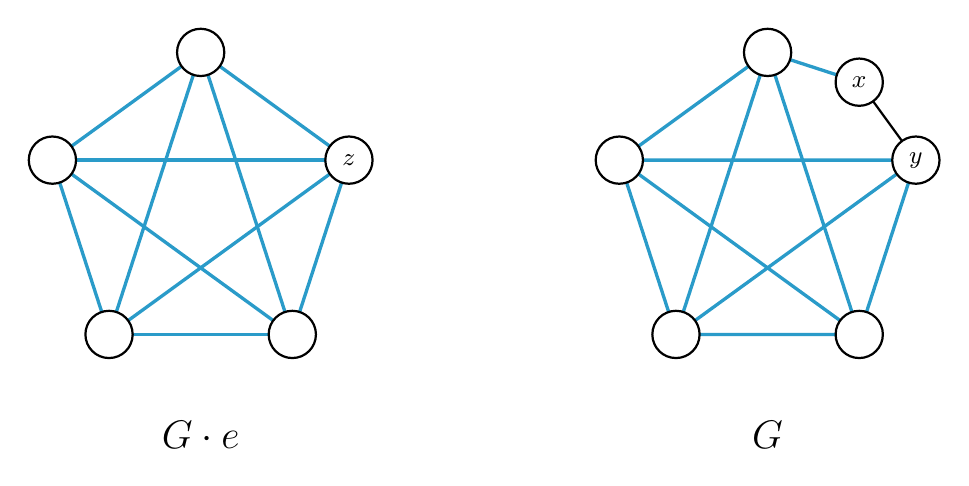
\begin{tikzpicture}[scale=0.9, auto, swap]
        % ================= 样式定义 (完全参照你的标准模板) =================
        \tikzset{
            % 节点样式:白底黑边圆圈
            vnode/.style={circle, draw=black, thick, fill=white, minimum size=6mm, inner sep=0pt, font=\small},
            % 蓝色路径样式 (代表细分路径,加重)
            blue_path/.style={very thick, cyan!80!black},
            % 黑色收缩边样式
            contract_edge/.style={thick, black}
        }

        % ================= 左图:G.e (z 是 K5 的分支顶点) =================
        \begin{scope}[shift={(-4,0)}]
            % 定义 5 个顶点位置
            \foreach \i in {1,...,5} {
                \coordinate (p\i) at (90 - 72*\i + 72:2.2);
            }

            % 绘制 K5 的 10 条蓝边
            \foreach \i in {1,...,4} {
                \pgfmathtruncatemacro{\ip}{\i+1}
                \foreach \j in {\ip,...,5} {
                    \draw[blue_path] (p\i) -- (p\j);
                }
            }

            % 绘制节点,将右上角节点标记为 z (p2)
            \foreach \i in {1,3,4,5} \node[vnode] at (p\i) {};
            \node[vnode] (z) at (p2) {$z$}; 

            \node at (0, -3.2) {\Large $G \cdot e$};
        \end{scope}

        % ================= 右图:G (x 在路径上,承担 1 个邻居) =================
        \begin{scope}[shift={(4,0)}]
            % 定义 5 个骨架顶点位置
            \foreach \i in {1,...,5} {
                \coordinate (q\i) at (90 - 72*\i + 72:2.2);
            }

            % 绘制骨架:1, 3, 4, 5 之间的 K4
            \draw[blue_path] (q1)--(q3) (q1)--(q4) (q1)--(q5) (q3)--(q4) (q3)--(q5) (q4)--(q5);
            
            % y (q2) 承担 3 个邻居:3, 4, 5
            \draw[blue_path] (q2)--(q3) (q2)--(q4) (q2)--(q5);

            % x 承担 1 个邻居:q1 (放置在 q2 到 q1 的路径上,54度方向)
            \coordinate (x_pos) at (54:2.2);
            \draw[blue_path] (x_pos) -- (q1);

            % 绘制黑色的收缩边 (不带 e 标注) 连接 x 和 y
            \draw[contract_edge] (x_pos) -- (q2);

            % 绘制节点
            \foreach \i in {1,3,4,5} \node[vnode] at (q\i) {};
            \node[vnode] (y) at (q2) {$y$};
            \node[vnode] (x) at (x_pos) {$x$};

            \node at (0, -3.2) {\Large $G$};
        \end{scope}

    \end{tikzpicture}
    \caption{如图是 $K_5$ 的情况,左图是细分之后,右图是未细分,蓝色是路径,黑色是边,如果 $x$ 仍然只够做路径上的分支,此时 $G$ 中有 $K_5$ 的细分}
\end{figure}

3. $x$ 在忽略到 $y$ 的连边后,向其它地方延伸出 2 条边; $y$ 在忽略到 $x$ 的连边后,向其它地方延伸出 2 条边,此时考虑原本 $K_5$ 中 $z$ 连向的四个分支顶点 $w_1,w_2,w_3,w_4$ ,不妨设 $x$ 连向 $w_1,w_2$ 而 $y$ 连向 $w_3,w_4$ ,考虑令左部点为 $\{x,w_3,w_4\}$ ,右部点为 $\{y,w_1,w_2\}$ ,构成 $K_{3,3}$ 的路径中,与 $x,y$ 有关的由题设保证,而 $w_1,w_2,w_3,w_4$ 内部路径的存在性由 $G\cdot e$ 中存在 $K_5$ 的子图保证,故 $G$ 中存在 $K_{3,3}$ 的细分。
\begin{figure}[H]
    \centering
    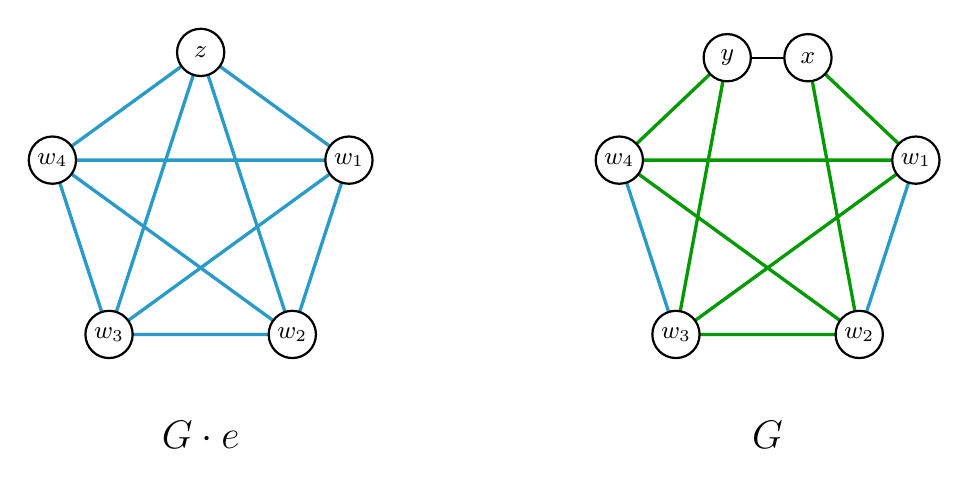
\begin{tikzpicture}[scale=0.9, auto, swap]
        % ================= 样式定义 (完全参照你的标准模板) =================
        \tikzset{
            % 节点样式
            vnode/.style={circle, draw=black, thick, fill=white, minimum size=6mm, inner sep=0pt, font=\small},
            % 蓝色路径 (非 K3,3 部分)
            blue_path/.style={very thick, cyan!80!black},
            % 绿色路径 (构成 K3,3 细分的部分)
            green_path/.style={very thick, green!60!black},
            % 黑色收缩边 (无标注)
            contract_edge/.style={thick, black}
        }

        % ================= 左图:G.e (z 是 K5 的分支顶点) =================
        \begin{scope}[shift={(-4,0)}]
            % 定义 5 个顶点位置 (z 在顶端,w1-w4 顺时针排列)
            \coordinate (z_p) at (90:2.2);
            \coordinate (w1_p) at (18:2.2);
            \coordinate (w2_p) at (306:2.2);
            \coordinate (w3_p) at (234:2.2);
            \coordinate (w4_p) at (162:2.2);

            % 绘制 K5 的 10 条蓝边
            \draw[blue_path] (z_p)--(w1_p) (z_p)--(w2_p) (z_p)--(w3_p) (z_p)--(w4_p);
            \draw[blue_path] (w1_p)--(w2_p) (w2_p)--(w3_p) (w3_p)--(w4_p) (w4_p)--(w1_p);
            \draw[blue_path] (w1_p)--(w3_p) (w2_p)--(w4_p);

            % 放置节点
            \node[vnode] at (z_p) {$z$};
            \node[vnode] at (w1_p) {$w_1$};
            \node[vnode] at (w2_p) {$w_2$};
            \node[vnode] at (w3_p) {$w_3$};
            \node[vnode] at (w4_p) {$w_4$};

            \node at (0, -3.2) {\Large $G \cdot e$};
        \end{scope}

        % ================= 右图:G (导出 K3,3 细分) =================
        \begin{scope}[shift={(4,0)}]
            % 定义 4 个骨架顶点
            \coordinate (w1) at (18:2.2);
            \coordinate (w2) at (306:2.2);
            \coordinate (w3) at (234:2.2);
            \coordinate (w4) at (162:2.2);
            
            % 将 z 拆分为 y (左) 和 x (右)
            \coordinate (y_pos) at (105:2.2);
            \coordinate (x_pos) at (75:2.2);

            % --- 1. 绘制不属于 K3,3 的蓝边 ---
            \draw[blue_path] (w1)--(w2);
            \draw[blue_path] (w3)--(w4);

            % --- 2. 绘制构成 K3,3 细分的绿边 ---
            % 左部点 {x, w3, w4}, 右部点 {y, w1, w2}
            % x 连向 y, w1, w2
            \draw[green_path] (x_pos)--(w1) (x_pos)--(w2);
            % y 连向 w3, w4 (x-y 连线见下方 contract_edge)
            \draw[green_path] (y_pos)--(w3) (y_pos)--(w4);
            % w3 连向 w1, w2
            \draw[green_path] (w3)--(w1) (w3)--(w2);
            % w4 连向 w1, w2
            \draw[green_path] (w4)--(w1) (w4)--(w2);

            % --- 3. 绘制黑色收缩边 (作为 K3,3 的一条路径) ---
            \draw[contract_edge] (x_pos) -- (y_pos);

            % 放置节点
            \node[vnode] at (w1) {$w_1$};
            \node[vnode] at (w2) {$w_2$};
            \node[vnode] at (w3) {$w_3$};
            \node[vnode] at (w4) {$w_4$};
            \node[vnode] at (y_pos) {$y$};
            \node[vnode] (x) at (x_pos) {$x$};

            \node at (0, -3.2) {\Large $G$};
        \end{scope}

    \end{tikzpicture}
    \caption{如图是 $K_5$ 的情况,左图是细分之后,右图是未细分,蓝色和绿色是路径,黑色是边,如果 $x$ 仍然只够做路径上的分支,此时 $G$ 中有 $K_{3,3}$ 的细分(只考虑绿色路径和黑色边)}
\end{figure}

因此这三种情况都可以让 $G$ 中存在一个 $K_5$ 或 $K_{3,3}$ 的细分。

因此我们分了 4 类 8 种情况,图的细分一定落在这些情况之中,而它们每一种都说明如果 $G\cdot e$ 含有 $K_{5}$ 或 $K_{3,3}$ 的细分作为子图,那么 $G$ 一定含有 $K_{5}$ 或 $K_{3,3}$ 的细分作为子图。

因此我们就说明了如果一个图 $G$ 不含有 $K_{5}$ 或 $K_{3,3}$ 的细分作为子图;那么 $G\cdot e$ 一定不含 $K_{5}$ 或 $K_{3,3}$ 的细分作为子图。

那么我们接下来可以归纳证明充分性了。

\section{充分性证明}
还记得我们一开始要找的最小反例图 $G$ 嘛?首先它显然是简单图。

我们在连通性归约部分证明了它一定是 3-连通的。

接下来我们说明它的顶点数必须不小于 5。

这是因为 $K_4$ ,作为唯一一个小于 5 个顶点的 3-连通简单图(因为点连通度不会大于度数最小的顶点的度数),它存在平面嵌入:

\begin{figure}[H]
    \centering
    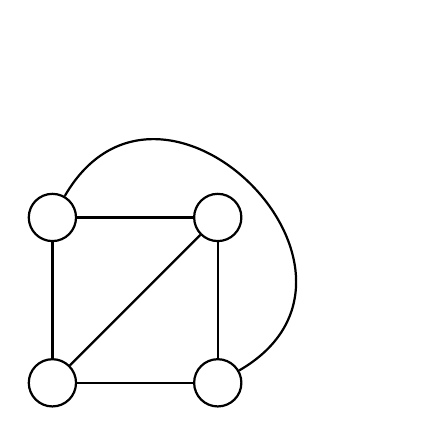
\begin{tikzpicture}[scale=0.7, auto, swap]
        % ================= 样式定义 (保持一致) =================
        \tikzset{
            % 节点样式:白底黑边圆圈
            vnode/.style={circle, draw=black, thick, fill=white, minimum size=6mm, inner sep=0pt, font=\small},
            % 连边样式
            edge/.style={thick, black}
        }

        % ================= 节点位置 (矩形布局) =================
        \node[vnode] (n1) at (-1.5, 1.5) {};
        \node[vnode] (n2) at (1.5, 1.5) {};
        \node[vnode] (n3) at (1.5, -1.5) {};
        \node[vnode] (n4) at (-1.5, -1.5) {};

        % ================= 连边 =================
        % 1. 外部矩形四边
        \draw[edge] (n1) -- (n2);
        \draw[edge] (n2) -- (n3);
        \draw[edge] (n3) -- (n4);
        \draw[edge] (n4) -- (n1);

        % 2. 内部对角线 (左下到右上)
        \draw[edge] (n4) -- (n2);

        % 3. 外部对角线 (左上到右下,画为外部圆弧以避免交叉)
        % 按照 image_2a4b45.png 所示,从上方绕行
        \draw[edge] (n1) to[out=60, in=30, looseness=2] (n3);

    \end{tikzpicture}
    \caption{如图,这是 $K_4$ 的平面嵌入}
\end{figure}

那么对于 $G$ ,既然它是点数不小于 5 的 3-连通图,我们在收缩引理部分证明了 $G$ 总存在一条边 $e$ 可以帮助它收缩得到一个 3-连通图 $G\cdot e$ ,在收缩性质部分证明了收缩得到的 3-连通图 $G\cdot e$ 不包含 $K_{5}$ 或 $K_{3,3}$ 的细分作为子图。

因此,由于 $G$ 是最小反例图,我们可以得出 $G\cdot e$ 是平面图,也就是它存在一个平面嵌入。

那么,我们最后要证明的就是,如果 $G$ 没有引入 $K_{5}$ 或 $K_{3,3}$ 的细分作为子图, $G$ 就是平面图。

那么怎么证明呢?不妨设 $G\cdot e$ 把原图的 $x,y$ 两个顶点收缩成 $z$ ,那么:

把 3-连通图 $G\cdot e$ 画在平面上,然后从中挖去 $z$ ,得到 $G\cdot e-\{z\}$ 的平面嵌入,注意,正是由于 $G\cdot e$ 是 3-连通的, $G\cdot e-\{z\}$ 是 2-连通的,也就是它不存在割点。

此时 $z$ 的原本位置一定在 $G\cdot e-\{z\}$ 的一个面 $f$ 上,我们考虑 $f$ 的边界,我们断言,正是由于 $G\cdot e-\{z\}$ 是 2-连通的,由于我们之前的推导,边界必定形成一个圈,也就是边界上的点和边形成的图,可以由一个简单回路点边不重复地遍历边界上的所有点和边。

那么我们就把这个回路找出来,不妨设为 $C=\{v_1,v_2,\cdots,v_n\}$ ,它由不同的顶点顺次连接而成,我们知道 $z$ 可以连接这些顶点,这个过程当然可以无交叉(就是 $G\cdot e$ 的画法嘛),但,对于原本的 $x,y$ ,这个过程可能就会引入交叉了。

\begin{figure}[H]
    \centering
    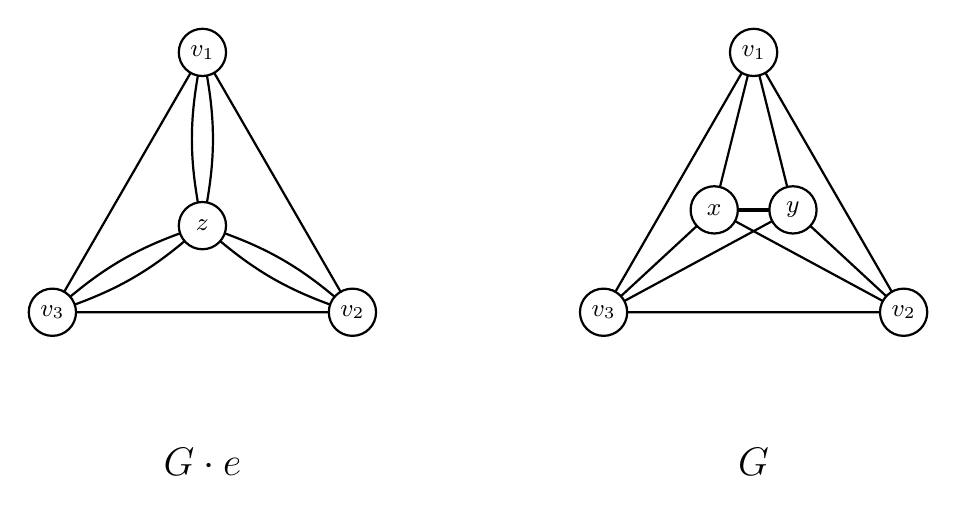
\begin{tikzpicture}[scale=1, auto, swap]
        % ================= 样式定义 =================
        \tikzset{
            % 节点样式:白底黑边圆圈
            vnode/.style={circle, draw=black, thick, fill=white, minimum size=6mm, inner sep=0pt, font=\small},
            % 全黑普通边样式
            edge/.style={thick, black}
        }

        % ================= 左图:G.e (收缩后的平面嵌入) =================
        \begin{scope}[shift={(-3.5,0)}]
            % 坐标定义 (保持三角形在外,体现环的特征)
            \coordinate (v1) at (90:2.2);
            \coordinate (v2) at (330:2.2);
            \coordinate (v3) at (210:2.2);
            \coordinate (z) at (0,0);

            % 绘制外圈环 (v1-v2-v3)
            \draw[edge] (v1) -- (v2) -- (v3) -- (v1);

            % 绘制 z 到 v1, v2, v3 的双重边 (体现原图 x,y 各自的连边合并)
            \foreach \target in {v1, v2, v3} {
                \draw[edge] (z) to[bend left=12] (\target);
                \draw[edge] (z) to[bend right=12] (\target);
            }

            % 放置节点并标注顺时针标号
            \node[vnode] at (v1) {$v_1$};
            \node[vnode] at (v2) {$v_2$};
            \node[vnode] at (v3) {$v_3$};
            \node[vnode] (zn) at (z) {$z$};

            \node at (0, -3) {\Large $G \cdot e$};
        \end{scope}

        % ================= 右图:G (K5 原始图) =================
        \begin{scope}[shift={(3.5,0)}]
            % 坐标定义 (与左图完全对齐)
            \coordinate (v1) at (90:2.2);
            \coordinate (v2) at (330:2.2);
            \coordinate (v3) at (210:2.2);
            % x 和 y 在内部横向排列,对应左图的 z 位置
            \coordinate (x_pos) at (-0.5, 0.2);
            \coordinate (y_pos) at (0.5, 0.2);

            % 绘制外圈环 (v1-v2-v3)
            \draw[edge] (v1) -- (v2) -- (v3) -- (v1);

            % 绘制 x 到 v1, v2, v3 的连线
            \draw[edge] (x_pos) -- (v1);
            \draw[edge] (x_pos) -- (v2);
            \draw[edge] (x_pos) -- (v3);
            
            % 绘制 y 到 v1, v2, v3 的连线
            \draw[edge] (y_pos) -- (v1);
            \draw[edge] (y_pos) -- (v2);
            \draw[edge] (y_pos) -- (v3);
            
            % 绘制待收缩的黑边 (稍微加粗以区分普通缩边)
            \draw[edge, ultra thick] (x_pos) -- (y_pos);

            % 放置节点
            \node[vnode] at (v1) {$v_1$};
            \node[vnode] at (v2) {$v_2$};
            \node[vnode] at (v3) {$v_3$};
            \node[vnode] at (x_pos) {$x$};
            \node[vnode] at (y_pos) {$y$};

            \node at (0, -3) {\Large $G$};
        \end{scope}

    \end{tikzpicture}
    \caption{该图直观展示了 $K_5$ (右)经过一次收缩操作把 $x-y$ 收缩为 $z$ 之后,变成了平面图(左,去掉重边等价于 $K_4$)}
\end{figure}

其中,我们可以观察到一些十分明显的可能情况。

\subsection{拥有不小于 3 个公共邻居}
不妨假设 $x,y$ 在 $C$ 上拥有不小于 3 个公共邻居,其中的三个是 \{u,v,w\} ,由于这三个顶点在回路 $C$ 上,这个回路本身就是 $u,v,w$ 互相可达的边不重复的路径(即提供了 $u\to v\to w\to u$ ),然后 $x,y$ 都与其它定点分别有连边,因此,这意味着 $G$ 有一个 $K_5$ 的细分作为子图。

\begin{figure}[H]
    \centering
    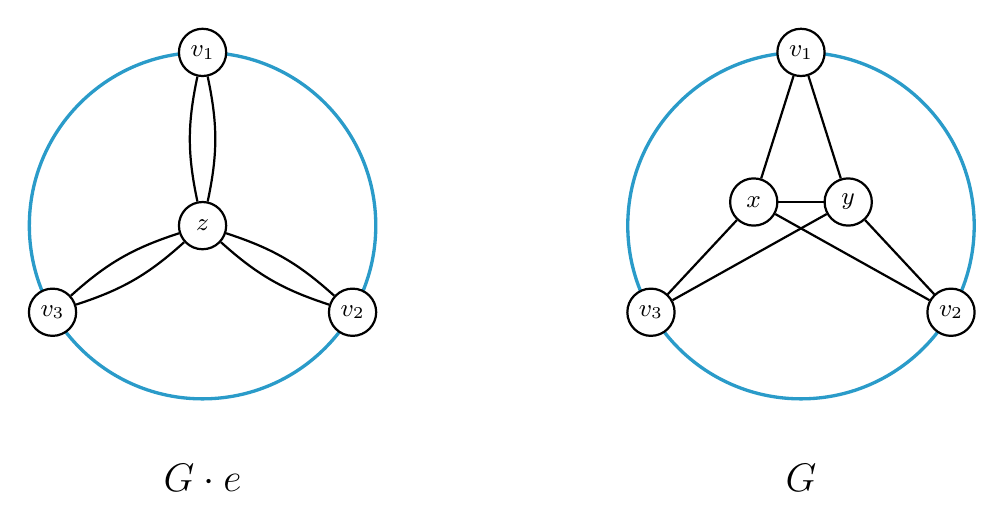
\begin{tikzpicture}[scale=1, auto, swap]
        % ================= 样式定义 (严格遵循你的最新要求) =================
        \tikzset{
            % 节点样式:白底黑边圆圈
            vnode/.style={circle, draw=black, thick, fill=white, minimum size=6mm, inner sep=0pt, font=\small},
            % 蓝色加重路径 (代表细分路径中的环路 C)
            blue_path/.style={very thick, cyan!80!black},
            % 全黑普通边样式 (不带 e 标注)
            edge/.style={thick, black}
        }

        % ================= 左图:G.e (z 是 x,y 合并后的点) =================
        \begin{scope}[shift={(-3.8,0)}]
            % 绘制外部环路 C (展示 v1, v2, v3 互相可达)
            \draw[blue_path] (0,0) circle (2.2);
            
            % 定义节点 (三角形位置)
            \node[vnode] (v1) at (90:2.2) {$v_1$};
            \node[vnode] (v2) at (330:2.2) {$v_2$};
            \node[vnode] (v3) at (210:2.2) {$v_3$};
            \node[vnode] (z) at (0,0) {$z$};

            % 绘制 z 到 v1, v2, v3 的双重边 (表示 x,y 共有邻居,收缩后合并)
            \foreach \target in {v1, v2, v3} {
                \draw[edge] (z) to[bend left=12] (\target);
                \draw[edge] (z) to[bend right=12] (\target);
            }

            \node at (0, -3.2) {\Large $G \cdot e$};
        \end{scope}

        % ================= 右图:G (引入 K5 细分) =================
        \begin{scope}[shift={(3.8,0)}]
            % 绘制外部环路 C
            \draw[blue_path] (0,0) circle (2.2);

            % 定义节点 (位置与左图完全对齐)
            \node[vnode] (v1) at (90:2.2) {$v_1$};
            \node[vnode] (v2) at (330:2.2) {$v_2$};
            \node[vnode] (v3) at (210:2.2) {$v_3$};
            
            % x, y 在内部,横向排列,对应左图的 z 位置
            \node[vnode] (x) at (-0.6, 0.3) {$x$};
            \node[vnode] (y) at (0.6, 0.3) {$y$};

            % 绘制连边:x, y 分别连向 v1, v2, v3 (公共邻居)
            \draw[edge] (x) -- (v1);
            \draw[edge] (x) -- (v2);
            \draw[edge] (x) -- (v3);
            
            \draw[edge] (y) -- (v1);
            \draw[edge] (y) -- (v2);
            \draw[edge] (y) -- (v3);
            
            % 绘制 x 到 y 的缩边 (黑色全黑,无标注)
            \draw[edge] (x) -- (y);

            \node at (0, -3.2) {\Large $G$};
        \end{scope}

    \end{tikzpicture}
    \caption{如图,蓝色线代表路径黑色线代表边,可以看到蓝色线(环路)其实已经让 $u,v,w$ 三个顶点两两连边了,因此引入 $K_5$ 也是非常自然的}
\end{figure}

那么由于 $G$ 是最小反例,它不可能拥有一个 $K_5$ 的细分作为子图,所以 $x,y$ 在 $C$ 上拥有的公共邻居个数不大于 2。

\subsection{拥有严格交替出现的邻居}
假设 $x,y$ 拥有严格交替出现的邻居,即 $x$ 拥有邻居 $u_1,u_2$ , $y$ 拥有邻居 $v_1,v_2$ ,且在回路上出现的次序是 $u_1,v_1,u_2,v_2$ ,那么既然这个回路提供了 $u_1\to v_1\to u_2\to v_2\to u_1$ 的路径(理解为 4 个顶点的环),然后 $x,y$ 都分别有连边,因此,设左部点为 $\{x,v_1,v_2\}$ ,右部点为 $\{y,u_1,u_2\}$ ,它们构成了一个 $K_{3,3}$ 的细分。

\begin{figure}[H]
    \centering
    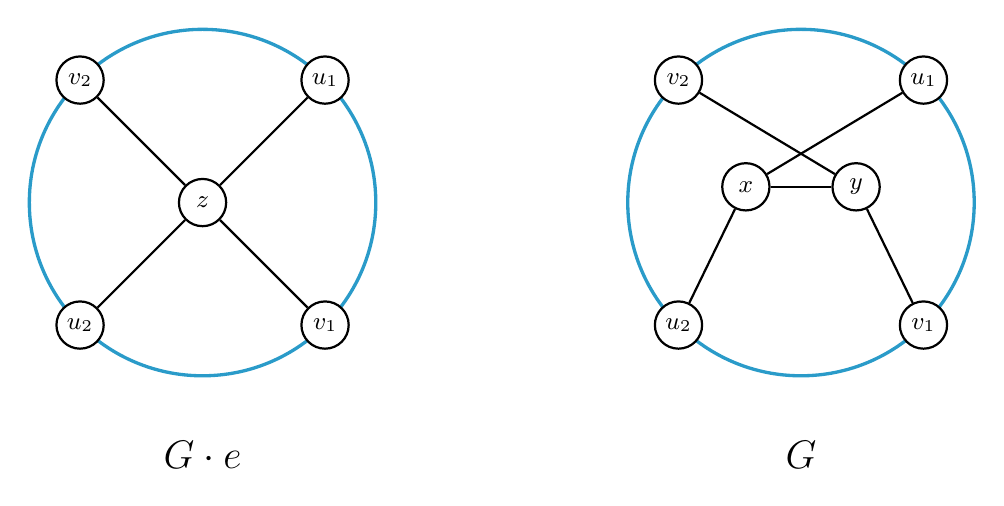
\begin{tikzpicture}[scale=1, auto, swap]
        % ================= 样式定义 (严格遵循你的标准模板) =================
        \tikzset{
            % 节点样式:白底黑边圆圈
            vnode/.style={circle, draw=black, thick, fill=white, minimum size=6mm, inner sep=0pt, font=\small},
            % 蓝色加重路径 (代表细分路径中的环路 C)
            blue_path/.style={very thick, cyan!80!black},
            % 全黑普通边样式 (不带 e 标注)
            edge/.style={thick, black}
        }

        % ================= 左图:G.e (收缩后的图) =================
        \begin{scope}[shift={(-3.8,0)}]
            % 绘制外部环路 C
            \draw[blue_path] (0,0) circle (2.2);
            
            % 定义四个邻居节点 (交替排列)
            \node[vnode] (u1) at (45:2.2) {$u_1$};
            \node[vnode] (v2) at (135:2.2) {$v_2$};
            \node[vnode] (u2) at (225:2.2) {$u_2$};
            \node[vnode] (v1) at (315:2.2) {$v_1$};
            
            % 收缩点 z 在中心
            \node[vnode] (z) at (0,0) {$z$};

            % z 继承 x, y 的所有邻居,连向四个点
            \draw[edge] (z) -- (u1);
            \draw[edge] (z) -- (v2);
            \draw[edge] (z) -- (u2);
            \draw[edge] (z) -- (v1);

            \node at (0, -3.2) {\Large $G \cdot e$};
        \end{scope}

        % ================= 右图:G (引入 K3,3 细分) =================
        \begin{scope}[shift={(3.8,0)}]
            % 绘制外部环路 C
            \draw[blue_path] (0,0) circle (2.2);

            % 定义节点 (位置与左图对齐)
            \node[vnode] (u1) at (45:2.2) {$u_1$};
            \node[vnode] (v2) at (135:2.2) {$v_2$};
            \node[vnode] (u2) at (225:2.2) {$u_2$};
            \node[vnode] (v1) at (315:2.2) {$v_1$};
            
            % x, y 在内部,横向排列
            \node[vnode] (x) at (-0.7, 0.2) {$x$};
            \node[vnode] (y) at (0.7, 0.2) {$y$};

            % 绘制连边:展示交替邻居带来的交叉
            % x 连向 u1 和 u2
            \draw[edge] (x) -- (u1);
            \draw[edge] (x) -- (u2);
            
            % y 连向 v1 和 v2
            \draw[edge] (y) -- (v1);
            \draw[edge] (y) -- (v2);
            
            % 绘制 x 到 y 的缩边
            \draw[edge] (x) -- (y);

            \node at (0, -3.2) {\Large $G$};
        \end{scope}

    \end{tikzpicture}
    \caption{如图,蓝色线代表路径黑色线代表边,可以看到蓝色线(环路)其实已经引入了 4 个顶点的偶环,再加上 $x,y$ 自然形成了 $K_{3,3}$ 的细分子图}
\end{figure}

那么由于 $G$ 是最小反例,它不可能拥有一个 $K_{3,3}$ 的细分作为子图,所以 $x,y$ 在 $C$ 上不会拥有严格交替的邻居。

\subsection{最后的准备}
我们尝试证明对于剩余的情况,总能导出 $G$ 的一个平面嵌入。

首先我们断言 $x$ 在 $C$ 上至少有两个邻居,这是好证明的,因为 $G$ 是 3-连通图,所以 $x$ 至少要连向 3 个不同的顶点,除去连向 $y$ 的还有两个都连在 $C$ 上;同理 $y$ 在 $C$ 上也至少两个邻居。

首先容易理解,只要导出了 $C\cup\{x,y\}$ 的平面嵌入,同时保持 $C$ 在原位,那么我们就可以导出整个图 $G$ 的一个平面嵌入。

好的那么能否导出 $C\cup\{x,y\}$ 的平面嵌入呢?又到了我们最喜欢的圈圈环节了!为了方便我们定义一下吧!

啊,好!对于 $C$ 我们任意指定一个遍历方向(比如顺时针),访问顺序是 $v_1\to v_2\to v_3\to \cdots\to v_n\to v_1\to \cdots$ ,对于 $C$ 上的任意两个不同的顶点 $u,v$ ,我们定义 $u$ 从顺时针遍历 $C$ 直到访问到 $v$ 的路径(包含点和边)为 $u$ 到 $v$ 的闭弧,记作 $[u,v]$ ;定义闭弧去掉 $u,v$ 端点为开弧 $(u,v)$ (可能不包含任何顶点),类似地,可以定义左开右闭弧和左闭右开弧,后面也会叫成区间,但它的本质是弧。

值得注意的是 $[u,v]$ 和 $[v,u]$ 只有端点重合; $[u,v]$ 和 $(v,u)$ 互补。

\subsection{弱区间引理}
弱区间引理的表述是,对于任意 $x$ 在 $C$ 上的两个邻居 $x_1,x_2$ ,或者使得全体 $y$ 在 $C$ 上的邻居都在 $[x_1,x_2]$ 上;或者使得全体 $y$ 在 $C$ 上的邻居都在 $[x_2,x_1]$ 上。

这是因为,假设它不成立,那么对于任意 $x_1,x_2$ ,取 $y_1\in (x_1,x_2)$ (否则所有点都属于 $[x_2,x_1]$ )和 $y_2\in (x_2,x_1)$ (否则所有点都属于 $[x_1,x_2]$ ),那么 $x_1,y_1,x_2,y_2$ 构成 $C$ 上交错序列,会导出 $K_{3,3}$ ,矛盾。

\begin{figure}[H]
    \centering
    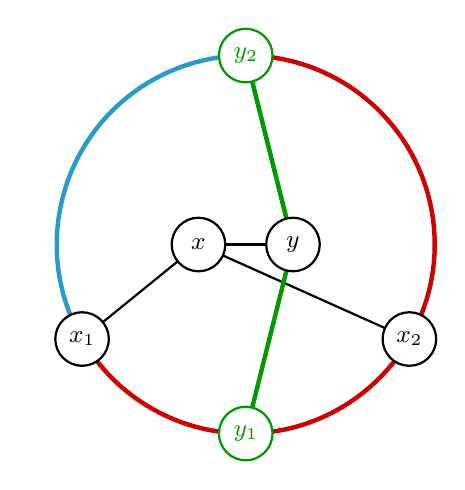
\begin{tikzpicture}[scale=1, auto, swap]
        % ================= 样式定义 (像素级复刻你的“标准”样式) =================
        \tikzset{
            % 标准白底黑边节点
            vnode/.style={circle, draw=black, thick, fill=white, minimum size=6.8mm, inner sep=0pt, font=\small},
            % 绿色虚拟节点样式 (用于 y1, y2)
            gnode/.style={circle, draw=green!60!black, thick, fill=white, minimum size=6.8mm, inner sep=0pt, font=\small, text=green!60!black},
            % 蓝色加重路径 (加重)
            blue_path/.style={ultra thick, cyan!80!black},
            % 红色加重路径 (加重)
            red_path/.style={ultra thick, red!80!black},
            % 绿色虚拟边 (加重)
            green_edge/.style={ultra thick, green!60!black},
            % 全黑普通边 (不带 e 标注)
            black_edge/.style={thick, black}
        }

        % ================= 坐标定义 (环在最外面,严格对称布局) =================
        \def\R{2.4}
        
        % 环上的邻居节点:按照交叉顺序排列 (y2, x2, y1, x1)
        \coordinate (y2_p) at (90:\R);   % 顶部 y2
        \coordinate (x2_p) at (330:\R);  % 右下 x2
        \coordinate (y1_p) at (270:\R);  % 底部 y1
        \coordinate (x1_p) at (210:\R);  % 左下 x1

        % 内部节点 x 和 y (模仿摆放位置)
        \coordinate (x_p) at (-0.6, 0);
        \coordinate (y_p) at (0.6, 0);

        % ================= 绘制环路 C (分段上色,确保在最外面) =================
        % 蓝色路径段:x1 到 y2 的短弧
        \draw[blue_path] (210:\R) arc (210:90:\R);
        % 红色路径段:y2 顺时针经过 x2, y1 回到 x1 的长弧
        \draw[red_path] (90:\R) arc (90:-150:\R);

        % ================= 绘制连边 (全黑/绿色路径) =================
        % 1. 内部核心黑边 x-y
        \draw[black_edge] (x_p) -- (y_p);
        
        % 2. x 的连边 (全黑)
        \draw[black_edge] (x_p) -- (x1_p);
        \draw[black_edge] (x_p) -- (x2_p);

        % 3. y 的虚拟连边 (绿色路径,对应 Caption 的虚拟边)
        \draw[green_edge] (y_p) -- (y1_p);
        \draw[green_edge] (y_p) -- (y2_p);

        % ================= 放置节点 (确保盖在路径上方) =================
        \node[vnode] at (x1_p) {$x_1$};
        \node[vnode] at (x2_p) {$x_2$};
        \node[gnode] at (y1_p) {$y_1$};
        \node[gnode] at (y2_p) {$y_2$};
        
        \node[vnode] at (x_p) {$x$};
        \node[vnode] at (y_p) {$y$};

    \end{tikzpicture}
    \caption{如图是弱区间引理的情况,蓝色和红色代表路径,黑色线代表边,绿色代表由反证假设出现的虚拟点边;如果假设弱区间引理不成立,红色路径标注了如何形成严格的交叉,由于我们之前已经告诉了这种交叉如何导出 $K_{3,3}$,这里不再说明}
\end{figure}

\subsection{强区间引理}
强区间引理的表述是,存在 $x$ 在 $C$ 上的两个邻居 $x_1,x_2$ ,满足 $x_1$ 的顺时针下一个满足是 $x$ 的邻居的第一个顶点就是 $x_2$,使得全体 $y$ 在 $C$ 上的邻居都在 $[x_1,x_2]$ 上。

这是因为,由弱区间引理,存在 $[x_1,x_2]$ 使得全体 $y$ 在 $C$ 上的邻居都在 $[x_1,x_2]$ 上,我们取包含边数最少的 $[x_1,x_2]$ ;如果 $x$ 只有两个邻居,命题显然成立。如果 $x_1$ 的顺时针下一个满足是 $x$ 的邻居的第一个顶点就是 $x_2$ ,命题也显然成立。

否则,不妨设 $x_1$ 的顺时针下一个满足是 $x$ 的邻居的第一个顶点是 $x_3$ ,此时 $x_2\ne x_3$ :

1. 如果 $[x_1,x_3)$ 没有任何 $y$ 的相邻顶点,那么 $[x_3,x_2]$ 是边数严格更少的满足条件的区间,与上一层(选取最少边)的反证假设矛盾。
2. 如果 $(x_3,x_2]$ 没有任何 $y$ 的相邻顶点,那么 $[x_1,x_3]$ 是边数严格更少的满足条件的区间,与上一层(选取最少边)的反证假设矛盾。

因此,我们证实了 $[x_1,x_3)$ 中和 $(x_3,x_2]$ 中都必然有 $x$ 的相邻顶点,继续讨论:

1. 如果 $(x_1,x_3)$ 中有任何 $y$ 的相邻顶点,那么取 $y_1\in (x_1,x_3),y_2\in (x_3,x_2]$ ,则 $x_1,y_1,x_3,y_2$ 交错,由于前面的推导,这会导出 $K_{3,3}$ 的细分子图,与外层反证假设( $G$ 不包含这种细分子图)矛盾。
2. 如果 $(x_3,x_2)$ 中有任何 $y$ 的相邻顶点,那么取 $y_1\in [x_1,x_3),y_2\in (x_3,x_2)$ ,则 $y_1,x_3,y_2,x_2$ 交错,由于前面的推导,这会导出 $K_{3,3}$ 的细分子图,与外层反证假设( $G$ 不包含这种细分子图)矛盾。

\begin{figure}[H]
    \centering
    % ================= 共有样式定义 =================
    \tikzset{
        % 标准白底黑边节点
        vnode/.style={circle, draw=black, thick, fill=white, minimum size=6.5mm, inner sep=0pt, font=\small},
        % 绿色虚拟节点 (x3)
        gnode/.style={circle, draw=green!60!black, thick, fill=white, minimum size=6.5mm, inner sep=0pt, font=\small, text=green!60!black},
        % 橙色分类节点 (实心小点,方便展示交叠)
        onode/.style={circle, draw=orange!80!black, thick, fill=orange!20, minimum size=4.5mm, inner sep=0pt, font=\scriptsize},
        % 加重路径
        blue_path/.style={ultra thick, cyan!80!black},
        red_path/.style={ultra thick, red!80!black},
        % 加重连边
        green_edge/.style={ultra thick, green!60!black},
        orange_edge/.style={ultra thick, orange!80!black},
        % 全黑普通边
        black_edge/.style={thick, black}
    }
    \def\R{2.4} % 统一半径

    % ================= 左图 (a): y1 in (x1,x3), y2 in (x3,x2] =================
    \begin{tikzpicture}[scale=1, auto, swap, baseline=(current bounding box.center)]
        \begin{scope}[shift={(-3.5,0)}]
            % 1. 坐标定义 (固化布局 210-270-330)
            \coordinate (x1_p) at (210:\R);
            \coordinate (x3_p) at (270:\R);
            \coordinate (x2_p) at (330:\R);
            % 顶部 y2 已移除

            % 橙色点坐标:
            % y1 严格在 (x1,x3) 内
            \coordinate (o1_p) at (240:\R);
            % y2 紧贴 x2 (相差 10 度,表现 [x3, x2] 的闭端点交叠)
            \coordinate (o2_p) at (320:\R); % 330 - 10 = 320

            % 内部点固化位置
            \coordinate (x_p) at (-0.6, 0);
            \coordinate (y_p) at (0.6, 0);

            % 2. 绘制环路 C
            \draw[blue_path] (330:\R) arc (330:570:\R); % 上方蓝弧
            \draw[red_path] (210:\R) arc (210:330:\R);  % 下方红弧 (活跃区)

            % 3. 绘制连边
            \draw[black_edge] (x_p) -- (y_p);
            \draw[black_edge] (x_p) -- (x1_p);
            \draw[black_edge] (x_p) -- (x2_p);
            \draw[green_edge] (x_p) -- (x3_p);
            % y 连向橙色点
            \draw[orange_edge] (y_p) -- (o1_p);
            \draw[orange_edge] (y_p) -- (o2_p);

            % 4. 放置节点 (注意覆盖顺序)
            \node[vnode] at (x1_p) {$x_1$};
            \node[vnode] at (x2_p) {$x_2$};
            \node[gnode] at (x3_p) {$x_3$};
            % 橙色点标注
            \node[onode] at (o1_p) {$y_1$};
            \node[onode] at (o2_p) {$y_2$}; % 紧贴 x2

            \node[vnode] at (x_p) {$x$};
            \node[vnode] at (y_p) {$y$};

            % 子图标题
            \node at (0, -3.5) {(a) $y_1 \in (x_1,x_3), y_2 \in (x_3,x_2]$};
        \end{scope}

    % ================= 右图 (b): y1 in [x1,x3), y2 in (x3,x2) =================
        \begin{scope}[shift={(3.5,0)}]
            % 1. 坐标定义
            \coordinate (x1_p) at (210:\R);
            \coordinate (x3_p) at (270:\R);
            \coordinate (x2_p) at (330:\R);
            % 顶部 y2 已移除

            % 橙色点坐标:
            % y1 紧贴 x1 (相差 10 度,表现 [x1, x3) 的闭端点交叠)
            \coordinate (o1_p) at (220:\R); % 210 + 10 = 220
            % y2 严格在 (x3,x2) 内
            \coordinate (o2_p) at (300:\R);

            % 内部点固化位置
            \coordinate (x_p) at (-0.6, 0);
            \coordinate (y_p) at (0.6, 0);

            % 2. 绘制环路 C
            \draw[blue_path] (330:\R) arc (330:570:\R);
            \draw[red_path] (210:\R) arc (210:330:\R);

            % 3. 绘制连边
            \draw[black_edge] (x_p) -- (y_p);
            \draw[black_edge] (x_p) -- (x1_p);
            \draw[black_edge] (x_p) -- (x2_p);
            \draw[green_edge] (x_p) -- (x3_p);
            % y 连向橙色点
            \draw[orange_edge] (y_p) -- (o1_p);
            \draw[orange_edge] (y_p) -- (o2_p);

            % 4. 放置节点
            \node[vnode] at (x1_p) {$x_1$};
            \node[vnode] at (x2_p) {$x_2$};
            \node[gnode] at (x3_p) {$x_3$};
            % 橙色点标注
            \node[onode] at (o1_p) {$y_1$}; % 紧贴 x1
            \node[onode] at (o2_p) {$y_2$};

            \node[vnode] at (x_p) {$x$};
            \node[vnode] at (y_p) {$y$};

            % 子图标题
            \node at (0, -3.5) {(b) $y_1 \in [x_1,x_3), y_2 \in (x_3,x_2)$};
        \end{scope}
    \end{tikzpicture}
    \caption{如图,蓝色和红色代表路径,黑色代表边,绿色代表由反证假设出现的虚拟点边;橙色代表由当前分类出现的虚拟点边,其中,橙色点与 $x_1$ 或 $x_2$ 的交叠的意思是它在 $[x_1,x_3)$ 的左闭右开弧或 $(x_3,x_2]$ 的左开右闭弧,即可能交叠;导致的交叉由红色路径标出}
\end{figure}

因此,我们证实了 $x_1,x_2$ 都必然与 $y$ 相邻,且 $(x_1,x_3)\cup (x_3,x_2)$ 中无顶点与 $y$ 相邻,继续讨论:

如果 $x_3$ 也与 $y$ 相邻,那么 $x_1,x_2,x_3$ 这三个顶点既与 $x$ 相邻又与 $y$ 相邻,由于前面的推导,这会导出 $K_5$ 的细分子图,与外层反证假设( $G$ 不包含这种细分子图)矛盾。

\begin{figure}[H]
    \centering
    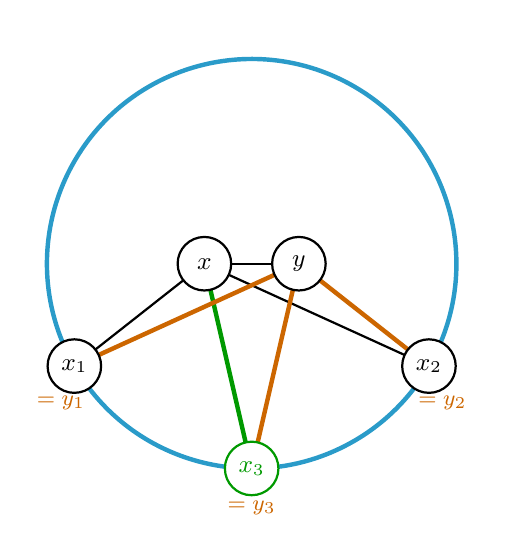
\begin{tikzpicture}[scale=1, auto, swap]
        % ================= 样式定义 (固化标准) =================
        \tikzset{
            % 标准白底黑边节点
            vnode/.style={circle, draw=black, thick, fill=white, minimum size=6.8mm, inner sep=0pt, font=\small},
            % 绿色虚拟节点 (x3)
            gnode/.style={circle, draw=green!60!black, thick, fill=white, minimum size=6.8mm, inner sep=0pt, font=\small, text=green!60!black},
            % 加重路径颜色
            blue_path/.style={ultra thick, cyan!80!black},
            red_path/.style={ultra thick, red!80!black},
            green_edge/.style={ultra thick, green!60!black},
            orange_edge/.style={ultra thick, orange!80!black},
            black_edge/.style={thick, black}
        }

        % ================= 坐标定义 (严格对齐 90-330-270-210 体系) =================
        \def\R{2.6}
        
        % 环上的关键点
        \coordinate (x1_p) at (210:\R);   % x1
        \coordinate (x2_p) at (330:\R);   % x2
        \coordinate (x3_p) at (270:\R);   % x3
        
        % 内部点 x, y (水平固化)
        \coordinate (x_p) at (-0.6, 0);
        \coordinate (y_p) at (0.6, 0);

        % ================= 绘制环路 C (蓝/红路径) =================
        % 蓝色长弧:非活跃区
        \draw[blue_path] (330:\R) arc (330:570:\R);
        % 红色短弧:活跃区间 [x1, x2]
        \draw[blue_path] (210:\R) arc (210:330:\R);

        % ================= 绘制连边 (黑/绿/橙) =================
        % 1. x 到 y, x1, x2 的黑边 (不带 e 标注)
        \draw[black_edge] (x_p) -- (y_p);
        \draw[black_edge] (x_p) -- (x1_p);
        \draw[black_edge] (x_p) -- (x2_p);
        
        % 2. x 到 x3 的绿边
        \draw[green_edge] (x_p) -- (x3_p);

        % 3. y 到 x1, x2, x3 的橙边 (即 y1, y2, y3)
        \draw[orange_edge] (y_p) -- (x1_p);
        \draw[orange_edge] (y_p) -- (x2_p);
        \draw[orange_edge] (y_p) -- (x3_p);

        % ================= 放置节点与子标签 =================
        % 环上主节点
        \node[vnode] at (x1_p) {$x_1$};
        \node[vnode] at (x2_p) {$x_2$};
        \node[gnode] at (x3_p) {$x_3$};
        
        % 橙色子标签:标注 =y1, =y2, =y3
        \node[orange!80!black, font=\footnotesize] at ($(x1_p)+(250:0.5)$) {$=y_1$};
        \node[orange!80!black, font=\footnotesize] at ($(x2_p)+(290:0.5)$) {$=y_2$};
        \node[orange!80!black, font=\footnotesize] at ($(x3_p)+(270:0.5)$) {$=y_3$};
        
        % 内部节点
        \node[vnode] at (x_p) {$x$};
        \node[vnode] at (y_p) {$y$};

    \end{tikzpicture}
    \caption{如图,蓝色和红色代表路径,黑色代表边,绿色代表由反证假设出现的虚拟点边;橙色代表由当前分类出现的虚拟点边,应当容易看出该分类会导出 $K_5$}
\end{figure}

因此,我们证实了 $x_1,x_2$ 都必然与 $y$ 相邻,且 $(x_1,x_2)$ 中无顶点与 $y$ 相邻,因此, $y$ 只有两个邻居在 $C$ 上,即 $x_1,x_2$ ,不妨设 $y_1=x_1,y_2=x_2$ 用来显示身份,因此显然 $y$ 的所有顶点也属于 $[x_2,x_1]$ ,继续讨论:

此时如果存在 $x$ 的邻居 $x_4$ 满足 $x_4\in(x_2,x_1)$ ,则 $y_1,x_4,y_2,x_3$ 交错,由于前面的推导,这会导出 $K_{3,3}$ 的细分子图,与外层反证假设( $G$ 不包含这种细分子图)矛盾。

\begin{figure}[H]
    \centering
    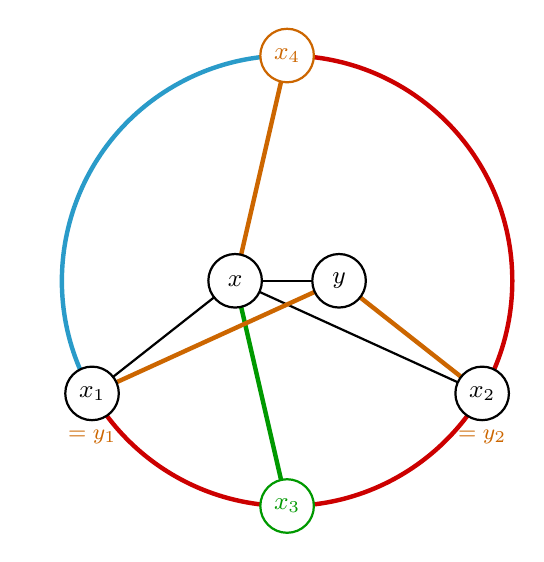
\begin{tikzpicture}[scale=1.1, auto, swap]
        % ================= 样式定义 (像素级复刻你的标准) =================
        \tikzset{
            % 标准节点
            vnode/.style={circle, draw=black, thick, fill=white, minimum size=6.8mm, inner sep=0pt, font=\small},
            % 绿色虚拟节点 (x3)
            gnode/.style={circle, draw=green!60!black, thick, fill=white, minimum size=6.8mm, inner sep=0pt, font=\small, text=green!60!black},
            % 橙色分类节点 (x4)
            onode/.style={circle, draw=orange!80!black, thick, fill=white, minimum size=6.8mm, inner sep=0pt, font=\small, text=orange!80!black},
            % 加重路径
            blue_path/.style={ultra thick, cyan!80!black},
            red_path/.style={ultra thick, red!80!black},
            green_edge/.style={ultra thick, green!60!black},
            orange_edge/.style={ultra thick, orange!80!black},
            black_edge/.style={thick, black}
        }
        \def\R{2.6}

        % ================= 坐标定义 (固化 90, 210, 270, 330 体系) =================
        \coordinate (x4_p) at (90:\R);   % 顶部 x4 (橙色)
        \coordinate (x1_p) at (210:\R);  % 左下 x1
        \coordinate (x3_p) at (270:\R);  % 底部 x3 (绿色)
        \coordinate (x2_p) at (330:\R);  % 右下 x2

        % 内部点 x, y (水平固化)
        \coordinate (x_p) at (-0.6, 0);
        \coordinate (y_p) at (0.6, 0);

        % ================= 绘制环路 C (分段上色) =================
        % 蓝色段:x1 到 x4 的左侧弧线
        \draw[blue_path] (210:\R) arc (210:90:\R);
        % 红色段:x4 顺时针经过 x2, x3 到 x1 的长弧线
        \draw[red_path] (90:\R) arc (90:-150:\R);

        % ================= 绘制连边 (谁连接了谁) =================
        % 1. 核心连接
        \draw[black_edge] (x_p) -- (y_p); % x-y 黑边

        % 2. x 的辐射连边 (黑/绿/橙)
        \draw[black_edge] (x_p) -- (x1_p);
        \draw[black_edge] (x_p) -- (x2_p);
        \draw[green_edge] (x_p) -- (x3_p);
        \draw[orange_edge] (x_p) -- (x4_p); % x 连向顶部的 x4

        % 3. y 的辐射连边 (橙色,指向 y1=x1, y2=x2)
        % 这两条橙色线会穿过 x 的黑色/绿色路径,视觉上直接导出 K3,3 交叉
        \draw[orange_edge] (y_p) -- (x1_p);
        \draw[orange_edge] (y_p) -- (x2_p);

        % ================= 放置节点与子标签 =================
        \node[onode] at (x4_p) {$x_4$};
        \node[vnode] at (x1_p) {$x_1$};
        \node[gnode] at (x3_p) {$x_3$};
        \node[vnode] at (x2_p) {$x_2$};
        
        % 橙色子标签 =y1, =y2
        \node[orange!80!black, font=\footnotesize] at ($(x1_p)+(270:0.5)$) {$=y_1$};
        \node[orange!80!black, font=\footnotesize] at ($(x2_p)+(270:0.5)$) {$=y_2$};

        % 内部节点
        \node[vnode] at (x_p) {$x$};
        \node[vnode] at (y_p) {$y$};

    \end{tikzpicture}
    \caption{如图,蓝色和红色代表路径,黑色代表边,绿色代表由反证假设出现的虚拟点边;橙色代表由当前分类出现的虚拟点边;导致的交叉由红色路径标出,应当容易看出这导出了 $K_{3,3}$}
\end{figure}

否则,$x_2$ 的顺时针下一个满足是 $x$ 的邻居的第一个顶点就是 $x_1$,与中层反证假设(强区间引理不成立)矛盾。

因此,在假设存在边数最少满足条件的 $[x_1,x_2]$ 的前提下,不论哪种情况都会导出矛盾,即第一层假设(存在最小边的选取)不成立,即不存在一个选取的边数是最小的。

但是由于满足条件的区间总数有限,且弱区间引理保证了满足条件的区间数目不为 0,又一定会存在至少一个边数最小的区间。

因此中层假设(强区间引理不成立)不成立,即强区间引理成立。

\subsection{最终证明}
强区间引理的证明其实标志着非平凡部分的结束,剩下的部分极其简单。

由强区间引理,一定存在 $x$ 的两个邻居 $x_1,x_2$ ,使得 $x$ 没有邻居属于 $(x_1,x_2)$ 且 $y$ 的全部 $C$ 上的邻居属于 $[x_1,x_2]$ 。

那么我们先随意摆放 $x$ ,然后将它与 $C$ 上的所有邻居连边,此时仍然是合法的平面嵌入,也就是说, $x$ 和 $x_1$ 的连边, $x$ 和 $x_2$ 的连边与 $[x_1,x_2]$ 这段弧会构成一个完整的面,不妨设为 $f_1$ 。

那么将 $y$ 放入这个 $f_1$ 内部,可以发现,由于 $y$ 的全部 $C$ 上的邻居属于 $[x_1,x_2]$ , $y$ 的全体邻居都在 $f_1$ 的边界上,此时,容易连边使得边不相交。

\begin{figure}[H]
    \centering
    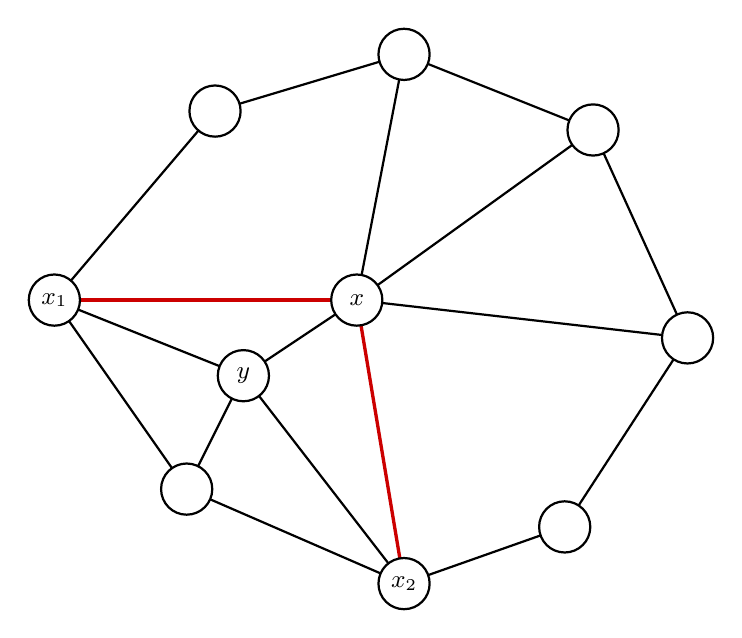
\begin{tikzpicture}[scale=1.2, auto, swap]
        % ================= 样式定义 (保持高度一致性) =================
        \tikzset{
            % 标准白底黑边节点
            vnode/.style={circle, draw=black, thick, fill=white, minimum size=6.5mm, inner sep=0pt, font=\small},
            % 黑色普通边
            black_edge/.style={thick, black},
            % 红色强调边 (x 连向 x1, x2)
            red_edge/.style={very thick, red!80!black}
        }

        % ================= 坐标定义 (拓扑布局复刻) =================
        % 外部多边形边界节点
        \coordinate (top) at (0.5, 2.8);
        \coordinate (tr) at (2.5, 2.0);
        \coordinate (r) at (3.5, -0.2);
        \coordinate (br) at (2.2, -2.2);
        \coordinate (x2_p) at (0.5, -2.8);   % x2
        \coordinate (bl) at (-1.8, -1.8);
        \coordinate (x1_p) at (-3.2, 0.2);   % x1
        \coordinate (tl) at (-1.5, 2.2);

        % 内部中心节点 x 和 y
        \coordinate (x_p) at (0, 0.2);
        \coordinate (y_p) at (-1.2, -0.6);

        % ================= 绘制连边 =================
        % 1. 外部环路 (黑色)
        \draw[black_edge] (top) -- (tr) -- (r) -- (br) -- (x2_p) -- (bl) -- (x1_p) -- (tl) -- (top);

        % 2. 内部节点 x 的连边
        \draw[black_edge] (x_p) -- (top);
        \draw[black_edge] (x_p) -- (tr);
        \draw[black_edge] (x_p) -- (r);
        \draw[black_edge] (x_p) -- (y_p);
        % x 连向 x1, x2 的红色强调边
        \draw[red_edge] (x_p) -- (x1_p);
        \draw[red_edge] (x_p) -- (x2_p);

        % 3. 内部节点 y 的连边 (根据强区间引理,全部落在 x-x1-x2 面内)
        \draw[black_edge] (y_p) -- (x1_p);
        \draw[black_edge] (y_p) -- (x2_p);
        \draw[black_edge] (y_p) -- (bl);

        % ================= 放置节点 =================
        % 外部节点
        \node[vnode] at (x1_p) {$x_1$};
        \node[vnode] at (x2_p) {$x_2$};
        \foreach \p in {top, tr, r, br, bl, tl} \node[vnode] at (\p) {};

        % 内部节点
        \node[vnode] at (x_p) {$x$};
        \node[vnode] at (y_p) {$y$};

    \end{tikzpicture}
    \caption{如图所示,强区间引理保证了我们可以先画出 $x$,然后把 $y$ 画在 $x-x_1-x_2$ 面上,从而给出合适的平面嵌入}
\end{figure}

由此我们给出了 $C\cup \{x,y\}$ 导出子图的平面嵌入,而其它部分只需要继承 $G\cdot e$ 的平面嵌入即可,因此,可以给出 $G$ 的平面嵌入,即 $G$ 是平面图。

但这与 $G$ 是最小反例矛盾。

因此 $G$ 存在的假设不成立。

因此,不存在一个最小的非平面图,满足它不包含 $K_5$ 或 $K_{3,3}$ 的细分子图。

因此,Kuratowski 定理的充分性成立。

又因为我们已经证明了 Kuratowski 定理的必要性。

Kuratowski 定理成立。

\section{尾声与吐槽}

所以说写到这里,我觉得你一定会明白为什么我会说我反引用的那篇文章是一篇具有误导性的教程。

具体而言,那篇文章的原文有如下表述“然后再删除 z 的邻居,直到删到图为可平面化为止,这时候得到一个包含 z 的区域”,这是非常不可原谅的错误,如果再删去邻居,图的 3-连通性会被破坏。

那篇文章的原文“因为图 G 是三通的,所以 G 缩边 Contraction 之后还是三通的”我看到这段话简直被气笑了,我用了 2000 多字严格证明,4 张图辅助理解的极其非平凡的引理,就被一笔带过。这个命题是极其不平凡的,而他的表述也是错误的,如果随意删边,3-连通性可能被破坏。

当然,其中还存在着位置漂移,充分性证明缺失等随意之处,不好判定是严重的逻辑硬伤还是作者用词不严谨导致的,我就不说了。

那篇文章的作者如果能够把自己引用权威背书时的详细程度拿出十分之一来用到他自己证明的严谨性上,也就不会有我这篇文章了。

不论如何,其实证明这个玩意是一件挺欢乐的事情,后续的许多更加优美的平面图有关的算法,很多时候也是基于类似的对平面嵌入的深刻理解展开的。

希望我的证明足够严谨,图解足够清晰,希望这篇文章对你有用,谢谢。

\vspace{2em}
\noindent\textbf{参考:} \\
\footnotesize
% 使用 \hypertarget{标签名}{内容} 定义跳转目标
\hypertarget{ref:csdn}{[1]} 某篇具有误导性的文章:\url{https://blog.csdn.net/m0_66201040/article/details/123440250}

\end{document}